\chapter{Experiment 2: Selection pressure}
\label{exp2}

\begin{figure}[hb]
    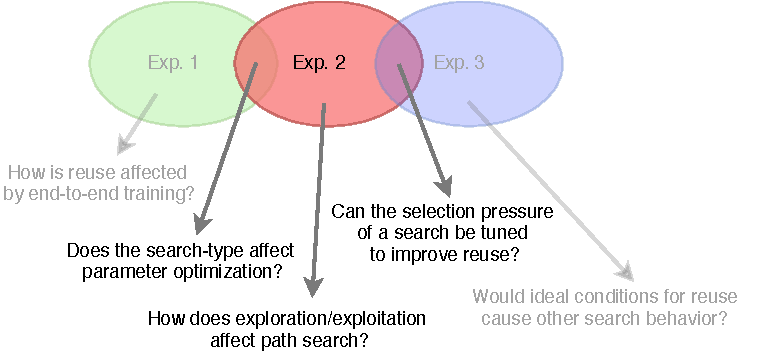
\includegraphics[width=\textwidth]{Chapters/4.Experiments/exp2/figures/exp2.pdf}
    \caption[Experiment focus]{Visualization of how the questions in this chapter fit in the larger context of this thesis.}
    \label{fig:exp2.questions}
\end{figure}

In the original paper, Fernando et al.\cite{pathnet} used a binary tournament search algorithm for path optimization. The algorithm was described as "the very simplest possible agent, a unit of evolution." Binary tournament search fits this description as a "unit of evolution" because it is the minimum change that can be done on a genome level to a population. Within one generation, the total change in the population is one genotype being replaced with another from the same population and subjected to mutation under some probability. Building on the previous set of experiments where the conclusion can take form as an argument in favor of a high exploration rate during path-search, we would expect a binary tournament search to yield modules with high transferability and a high number of module reuse compared to a high exploitation algorithm. In these experiments, this will be tested by manipulating the selection pressure of each search. Questions addressed in this chapter is: 
\begin{itemize}
    \item \emph{Does favoring either exploration or exploitation influence module reuse?}
    \item \emph{How does different selection pressure schemes impact path search and learning?}
\end{itemize}


\section{Description}
\label{exp2:description}
\subsection{Data-sets} 
\label{exp2:datasets}
To address these questions, a trial of different searches have been applied to a PathNet structure for a selection of tasks. As with the first-path experiments, the search algorithms will be applied to image classification tasks. Building on what we learned with regards to task difficulty, two different data-sets have been selected, and the different tasks will be derived from this data. The tasks will be ordered by the assumed difficulty to follow a gradual learning mentality. 

\begin{enumerate}
    \item MNIST subtasks
    \begin{enumerate}
        \item Digits 0, 1, 2, 3 and 4
        \item Digits 5, 6, 7, 8 and 9 
    \end{enumerate}
    \item Full MNIST classification
    \item cSVHN subtasks
    \begin{enumerate}
        \item Digits 0, 1, 2, 3 and 4
        \item Digits 5, 6, 7, 8 and 9 
    \end{enumerate}
    \item Full cSVHN classification
\end{enumerate}

It was shown during the first-path experiments that task 1a and 1b is not of the same difficulty level, however, within this context we will consider the training amount needed to reach a satisfactory accuracy level is similar enough for these tasks to be grouped. The natural progression from a full MNIST classification to  SVHN is thought to increase the incentive for module reuse, even if the SVHN task will have to learn to ignore distractions in the images (see \ref{Implementation:SVHN}) that the MNIST classifiers do not have to deal with. The difference in image-dimensions has been addressed in \ref{exp2:implementation}.

As mentioned in \ref{Implementation:SVHN} there are two formats to the SVHN set, one of variable image resolutions, and one that mimics the MNIST set in static square size called cropped SVHN (cSVHN). cSVHN is selected for these experiments to use a constant input size to the PathNet. Within the comprehensive set of cSVHN images, a subset described as containing "somewhat less difficult samples" is used in this chapter. To increase the number of tasks in the future, the rest of the SVHN data could be used, and noise could be added to the images to raise the task difficulty artificially. 

For both the MNIST and cSVHN set, the amount of training data have been limited to 10000 training samples and 4000 validation samples. Of these samples, MNIST have a fairly even distribution on each class while SVHN have an imbalance in the class distribution. Since the samples used are randomly selected before each experimental run, the probability of selecting one sample from a given class can be derived from the total amount of samples in that class (see \ref{Implementation:SVHN} for the exact number of samples in each class).

Each experimental run will apply a searching scheme to find an optimal path in a gradually increasing knowledge base within a PathNet. This means, for instance, tasks 1a always will be learned in a module-set of only initialized weights and no previous knowledge. 
\begin{enumerate}
    \item Constant selection pressure
    \begin{enumerate}
        \item Tournament size 2
        \item Tournament size 25
        \item Tournament size 3 + recombination
    \end{enumerate}
    \item Scaling selection pressure
    \begin{enumerate}
        \item Low to high pressure: 2, 5, 10, 15, 20, 25
        \item High to low pressure: 25, 20, 15, 10, 5, 2
    \end{enumerate}
    \item Dynamic selection pressure
    \begin{enumerate}
        \item Gradual change from 2 to 25 during each search
        \item Gradual change from 25 to 2 
    \end{enumerate}
\end{enumerate}
In total, the seven tournament algorithms are used ten times each within a reinitialized PathNet structure to train on all tasks discussed in \ref{exp2:datasets}. Between algorithms, the only hyper-parameter change is the tournament size and replacement method within each tournament. All algorithms except 1c use a winner-replace-all scheme where the mutation of the strongest paths genome replaces each of the losing contenders in the tournament. In algorithm 1c, three contenders are selected randomly from the population and evaluated. The two strongest genomes are labeled as parents and (starting with the winner) takes turns copying their layers to the offspring. The offspring are then subject to some mutation under the same probability as every other algorithm and replaces the losing genome in the tournament.
\begin{figure}[ht]
    \centering
    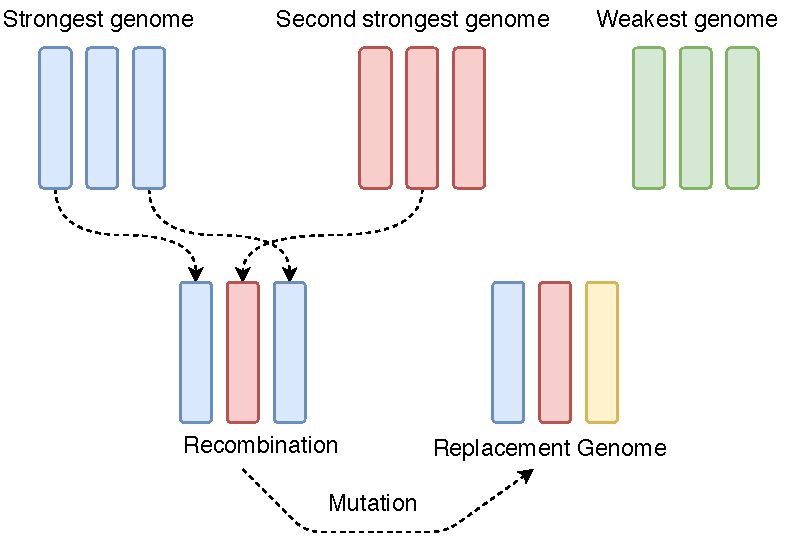
\includegraphics[width=0.8\textwidth]{Chapters/4.Experiments/exp2/figures/Recombination_algorithm.pdf}
    \caption[Recombination algorithm]{Visualization of the recombination in algorithm 1c. In a three-layer PathNet, the first and last layer in the recombination would be layer one and three in the winning genome, while layer two would stem from the second strongest genome. After a mutation of the recombination, the new genome replaces the losing contender. Each color represents one genome from the tournament, and yellow represents a mutation.}
    \label{fig:search.recombination_algorithm}
\end{figure}

Algorithm group 2 consists of two algorithms where the tournament size is changed between each task. This means algorithm 2a uses tournament size 2 for task 1a, task 1b uses tournament size 5 and so on until the last task of full cSVHN classification which uses tournament size 25. In algorithm 2b, this order of tournament sizes is reversed. It is expected that in the visualization of metrics where a population average is calculated for each generation, such as training accuracy, an algorithm with high selection pressure will have abrupt value changes from one generation to the next. Low selection pressure would then give a more gradual change in such values. A change between these two curve types should be prominent for algorithms 2a and 2b.

Algorithms 3a and 3b have its selection pressure changed during each tournament search. This means each algorithm behave the same for each task, which algorithms 2a and 2b did not. The change in selection pressure is gradual which means between tournament sizes 2 and 25; each tournament size is used about four times for a search termination limit of 100 generations. It is evident that an even distribution of tournament sizes on each generation is not possible when using a threshold accuracy as search termination, which is one reason searches in these experiments are limited by the number of generations instead. 

\subsection{Metrics}
\label{exp2:metrics}

\subsubsection{Modular reuse}
As with the first-path experiments, module reuse between tasks will be an important metric for these experiments. One unit of modular reuse is counted if a path contains a pre-trained module. In a multi-task scenario with more than two tasks, a module might be reused in more than one path and are in those cases counted once for each path reusing it. When discussing the properties of each algorithms modular reuse, it is the cumulative reuse for each task that is used.

Modular reuse is assumed to be an appropriate metric to describe the transferability of the knowledge a module acquire during training. It is also assumed that modules are able to contain some form of "memetic"\footnote{Memetic is used here to describe a quantification of knowledge in the same way "meme" is used by Richard Dawkins\cite{selfishGene} to describe a unit of cultural knowledge, here as a unit of knowledge used to solve a task.} unit knowledge

\subsubsection{Capacity use}
Highly correlated to reuse, the total amount of modules used (capacity) provides a measure of how efficiently the possible parameters are used for each task. The complexity a classifier is capable of describing is governed by the amount of available capacity in that classifier, where capacity is the amount of tunable\footnote{Here the capacity used by a path can include locked modules, which make them non-tunable.} parameters allocated to the task.

\subsubsection{Validation accuracy}
When discussing classifiers, validated classification accuracy is a natural metric to discuss. However, under these circumstances, the accuracy will be affected by the training amount, which is changing across algorithms. Accuracy will, therefore, be viewed in the context of the total amount of training units applied to each path. The definition of a training unit is described in section \ref{background:pathnet.search}.

\subsubsection{Population diversity}
The change in population diversity during each search will be used to rank each algorithm by its selection pressure as it should provide a clear indication of an algorithms convergence rate. As discussed in section \ref{background:diversity}, both pair-wise Hamming distance and unique genome frequency will be used.

\section{Hypothesis}
\label{exp2:hypothesis}
The expectations for these experiments were heavily influenced by the results of the first-path experiments in chapter \ref{exp1}. When the training algorithms are viewed in a simplified context of only "exploration vs. exploitation," we can place them on a scale between these extremes and discuss expected outcomes from each end of the spectrum. In this context, the Pick+Search learning scheme used in the first-path experiments would fall on the exploitation side as only one permutation of modules is tried.

Regarding tournament size, it is expected that the searches using lower tournament sizes have a lower selection pressure than algorithms using a high tournament size. This is a natural assumption to make considering the changes made to a population in each generation. Algorithms using a winner-replace-all\ref{implementation.search} replacement scheme change all genomes that is a part of the tournament except for the winner, which means the larger tournament sizes causes a larger change in the overall population. The winner of a large tournament is more favored than the winner of a smaller tournament, making the pressure for being selected (winning) higher. 

During a search, a populations diversity shifts from an initialized state of high diversity towards a lower diversity where some optimal path can be found. As discussed, a large tournament size causes rapid changes in a population compared to a low tournament size, where the diversity drops from one generation to the next when the winning genome is duplicated. This rate at which a population converges toward a low diversity is therefore expected to be highly correlated to the tournament size.

A population is said to have converged when the diversity can not feasibly be reduced further due to mutation. Each tournament after that point would only consist of small mutations of the same genotype, making the search performing something on the order of end-to-end training as seen in the previous experiment. 

\begin{figure}[ht]
    \centering
    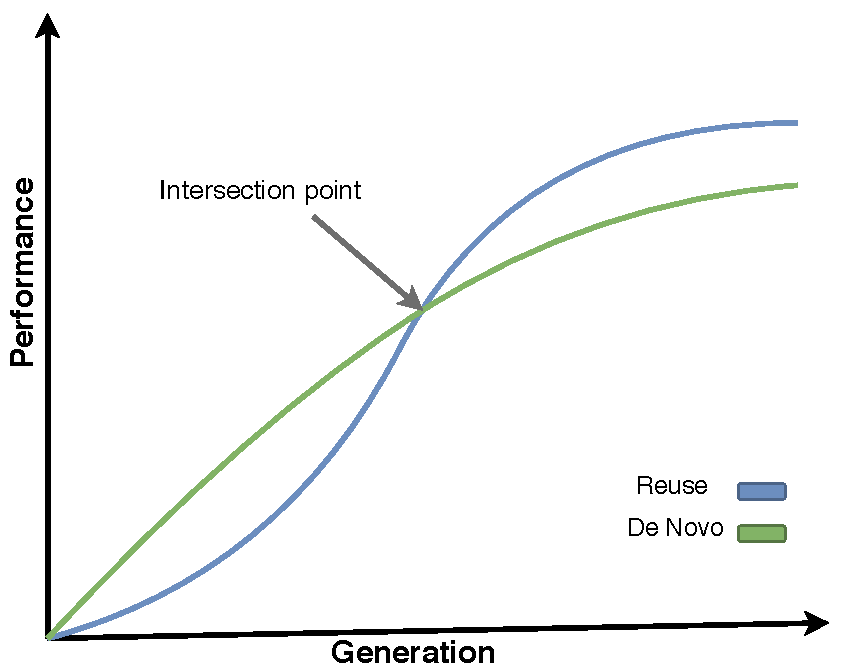
\includegraphics[width=0.8\textwidth]{Chapters/4.Experiments/exp2/figures/reuse_vs_new.pdf}
    \caption[Hypothetical performance plot]{A hypothetical plot of performance changing during a search. The two curves represent the performance of two paths where one have a lot of reuse(blue) and the other train all modules \textit{de novo}(green). The point at which reuse becomes advantageous is marked as "intersection point".}
    \label{fig:reuse_vs_new}
\end{figure}

In chapter \ref{exp1}, task difficulty was used to explain why searches resulted in using less pre-trained modules than if modules were selected randomly. We can use this effect as a definition of a task being too simple. For a scenario training on a such a task, performance of a path consisting of modules being trained \textit{de novo} would improve quicker than the performance of a path with a lot of reuse. A hypothetical scenario is plotted in figure \ref{fig:reuse_vs_new} where it is easier to train new module than learning the interface of locked modules. If the selection pressure of an algorithm is low enough for the population to converge before the intersection point between the two performance curves, training new modules from scratch would be seen a heavily favored by the algorithm.  Algorithms that converge after that point would have a higher likelihood of reusing modules as they have enough "search time" to learn the locked module interfaces. A high selection pressure algorithm with a rapid convergence will have a higher likelihood of converging before the intersection point, and we would, therefore, expect it to have a lower reuse than algorithms with a low selection pressure. 

Each path taking part in a tournament is trained and evaluated, meaning searches with a high tournament size will train its modules more for each generation than searches with a low tournament size. Algorithm 1b which throughout the multi-task scenario has the highest tournament size is therefore expected to reach the highest validation accuracy among the algorithms tried, followed by algorithms 3a and 3b with a total amount of evaluations of 1317 evaluations during 100 generations. The low tournament size algorithms 1a and 1c, the least amount of evaluations and the accuracy, is expected to reflect that. Algorithms 2a and 2b change between the maximum and minimum set tournament sizes and we expect them to therefore gradually change accordingly.

\section{Experimental setup}
\label{exp2:implementation}

\subsection{PathNet}
The PathNet structure used for these experiments have three layers of 20 modules where each path may contain one, two or three modules in each layer. Six optimal paths with maximum 3 active modules for a given layer calls for a PathNet structure of at least 18 modules in each layer. By setting the PathNet dimensions to 3-by-20, there is enough capacity to assign the maximum amount of modules to each task without any overlap.

% Please add the following required packages to your document preamble:
% \usepackage{multirow}
\begin{table}[ht]
\centering
\begin{tabular}{llc}
PathNet depth            & \multicolumn{2}{c}{3}               \\
PathNet width            & \multicolumn{2}{c}{20}              \\
Maximum active modules   & \multicolumn{2}{c}{3}               \\
MaxPooling               & \multicolumn{2}{c}{2x2}             \\
Task optimizer           & \multicolumn{2}{c}{Adam}            \\
Learning rate            & \multicolumn{2}{c}{0.001}           \\
Loss function            & \multicolumn{2}{c}{Crossentropy}    \\
\multirow{7}{*}{Modules} & Type                & Convolutional \\
                         & Layers              & 1             \\
                         & Channels            & 2             \\
                         & Kernel              & 3x3           \\
                         & Stride              & 1x1           \\
                         & Activation          & ReLU          \\
                         & Batch Normalization & Yes           \\
\end{tabular}
\caption[Selection pressure experiment hyper-parameters]{Hyper parameters used during the selection pressure experiments.}
\label{tab:exp2.hyperparams}
\end{table}

As with the refined first-path experiments, only convolutional modules with ReLU activation were used, but with two channels each instead of the one in first-path. To verify, a random path with these hyper-parameters were created and applied to the task of full cSVHN classification and was able to reach a satisfactory performance within a reasonable training time. The Adam optimizer was used during backpropagation with a learning rate of 0.0001. A full list of hyperparameters used can be found in table \ref{tab:exp2.hyperparams}. 

Each convolutional module also includes a batch-normalization operation, and the last modules end in a max-pooling before the output is flattened and passed through the final unique classification layer. 

\subsection{Image-sets}
As there is a resolution difference between the cSVHN set and MNIST, an additional preprocessing step was applied to the MNIST set. A 2-pixel border of zeros was added to change the dimensions from 28x28 to 32x32. cSVHN images have three-channels of RGB values, so the single channel of padded MNIST images was repeated in every color-channel to reach the final dimensions of 32x32x3.  

\begin{figure}[ht]
    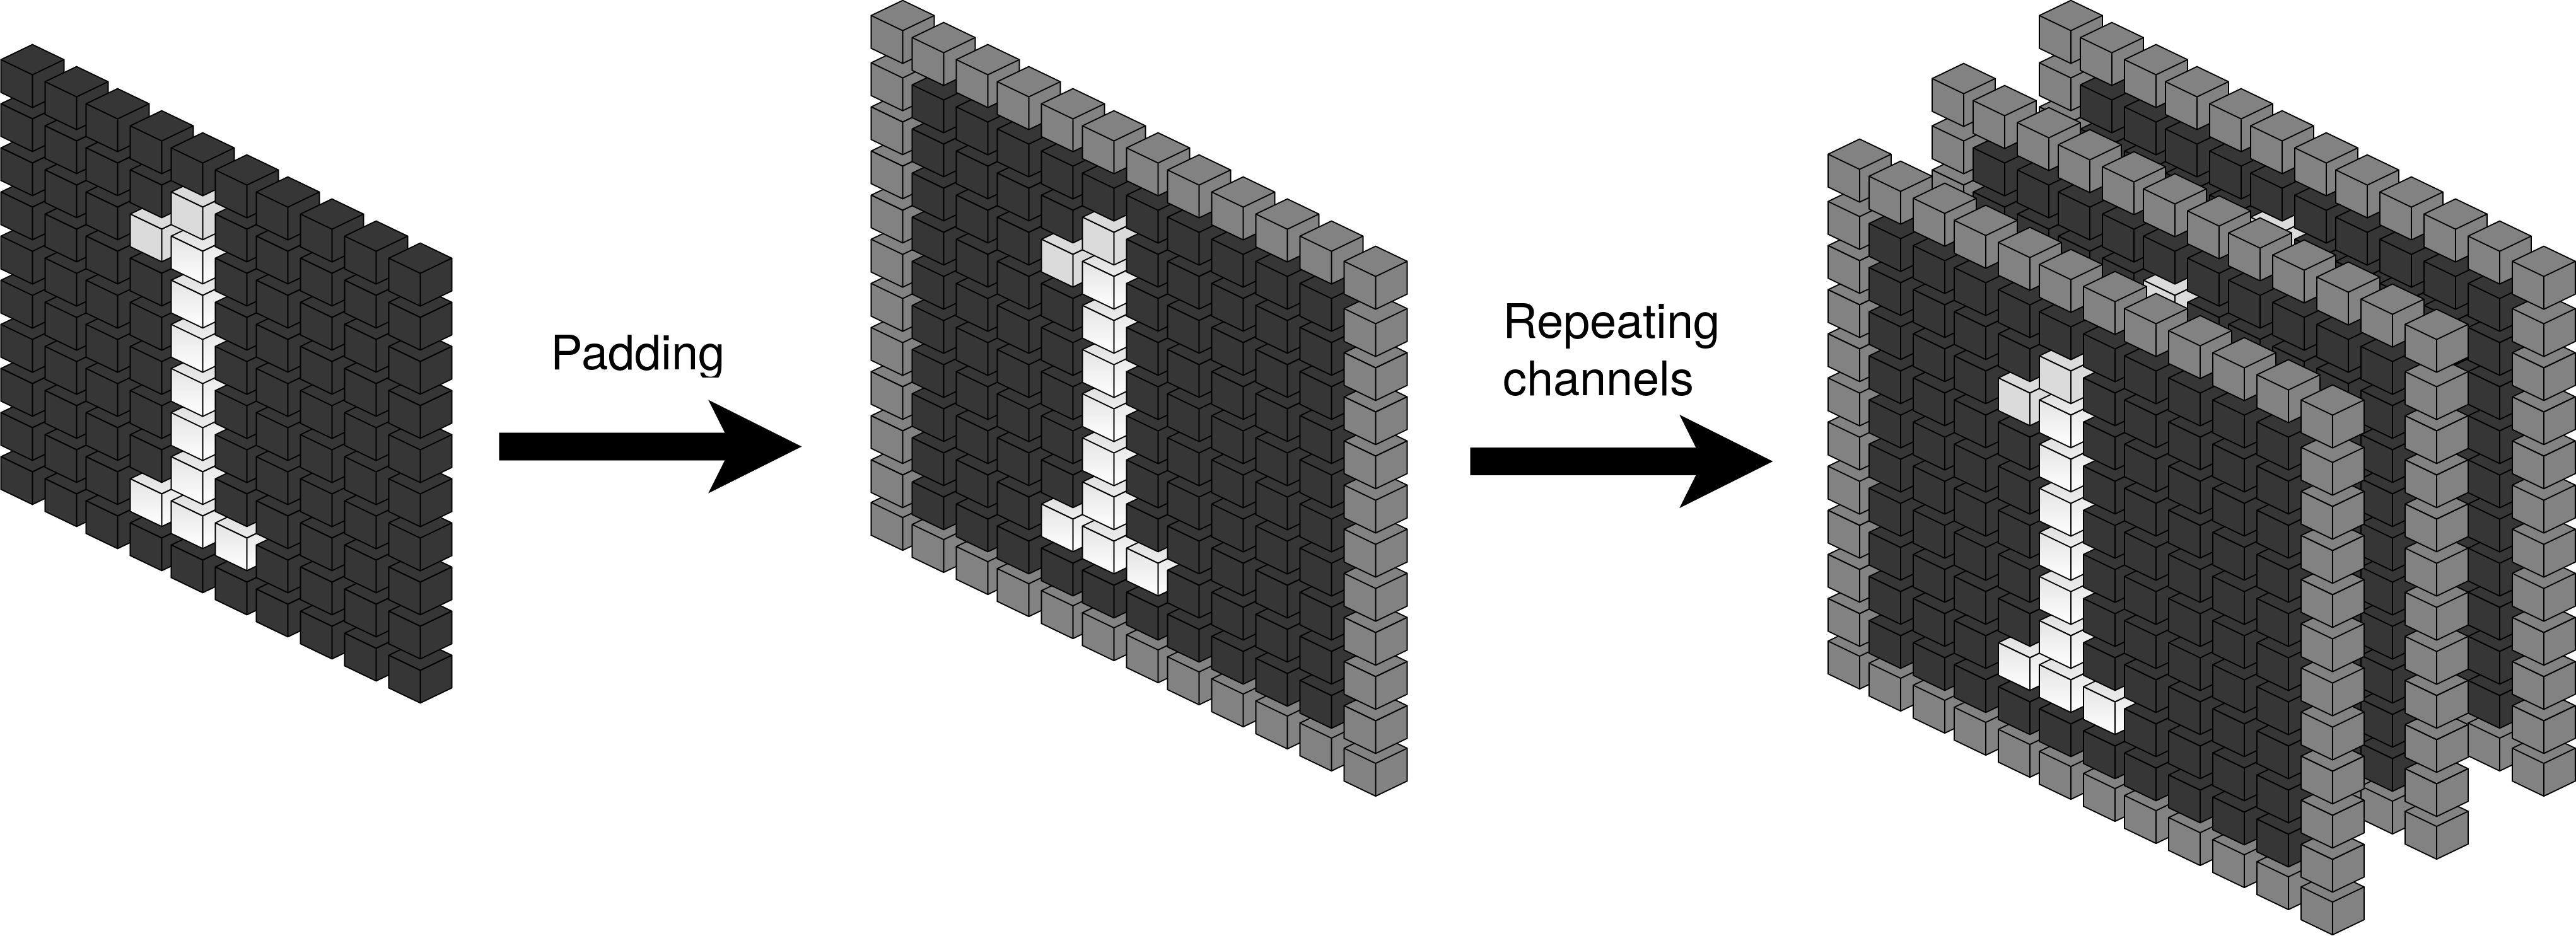
\includegraphics[width=\textwidth]{Chapters/4.Experiments/exp2/figures/MNISTpadding+repeating.png}
    \caption[MNIST modifications]{How MNIST is adapted to have same dimensions as cSVHN. Illustration use dimensions 12x12x3 while cSVHN and adapted MNIST use 32x32x3}
    \label{fig:MNISTpadding}
\end{figure}

\subsection{Tournament Search}\label{exp2:implementation.search}
The tournament search uses a population size of 64, and as discussed, a winner-replaces-all replacement scheme between generations. Instead of using a accuracy threshold as in the previous experiments, the search terminates after 100 generations. An important feature of PathNet is the way learning is done. Since network backpropagation occurs during path fitness-evaluation, the locked number of generations limit the amount of training that is allowed. In the original paper, fitness is set as the negative training error which is reached for each path after it has been trained for one training unit of 50 mini batches of size 16. This is a reasonable way of evaluating the fitness of a path when using a small tournament size, but as the tournament size have been increased tenfold for the algorithms with high selection pressure, fitness is calculated differently in these experiments. 

The problem of directly using the training error as fitness is that the error changes whenever weights along a path are updated. An extreme example can be used to present the underlying problem with this.

\begin{figure}[ht]
    \centering
    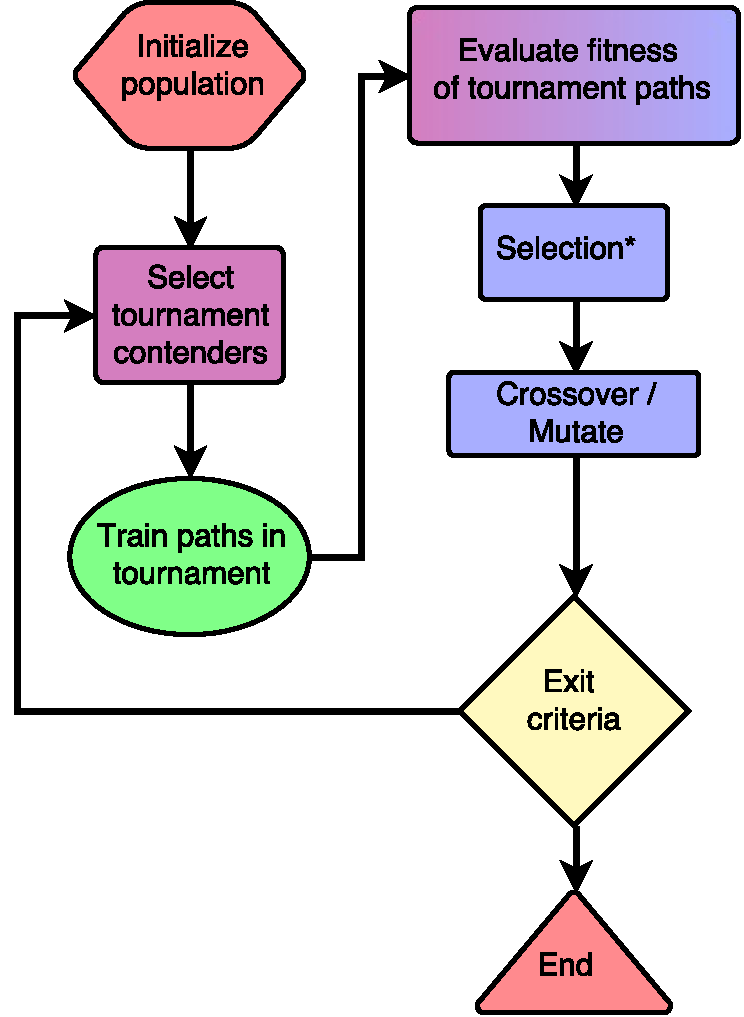
\includegraphics[width=0.5\textwidth]{Chapters/4.Experiments/exp2/figures/TS_implementation.pdf}
    \caption[Tournament search flowchart]{Flowchart of the tournament search implemented here. Compared to the flowchart of standard Tournament Search implementation in figure \ref{fig:algorithmflowcharts}, the difference is the extra step of training (green) before the fitness is evaluated. *The selection function always selects the tournament winner, except during algorithm 1c where the top two paths is selected.}
    \label{fig:ts_flowchart}
\end{figure}

Take a tournament selection of 25 genomes containing 24 identical paths and one different path with some module overlap to the others and which is evaluated first. One scenario could be that the first unique path is evaluated to a high fitness, when the next path evaluated, the weights in the modules which overlap between the two are updated. The evaluated fitness of the first path is now outdated, and for every subsequent path, this fitness might get worse and worse if the parameters in the overlapping modules move to an area of high error in the context of the first paths other modules. After all fitness evaluations, the first path now stands with a high fitness, which might be larger than that of all other paths in the tournament. Then all other paths in the tournament are replaced with the winning path even if its actual fitness might have become significantly reduced during the evaluation step. Due to this, the fitness of paths in a tournament is calculated in a separate step for these experiments as seen in figure \ref{fig:ts_flowchart}. After a subset of the population is selected for a tournament, all paths in that tournament are trained for one training unit. When training is completed, each path is evaluated by using a new subset of the training data for validation. This way, the order in which paths are validated does not affect the fitness score, which is the classification accuracy reached during the validation step. The order of paths still affect the training, but the fitness used for selecting a tournament winner is the "true"\footnote{Fitness is calculated on the basis of the training data-set, which means it might become overly optimistic over time. Overfitting during training is discussed in the context of another experiment} fitness score.

The same reason influence the final step of the tournament search. When the limit of a hundred generations is reached, all paths in the population is evaluated again. Since the true fitness of a path might change from one generation to the next, only the paths participating in the final tournament has its true fitness score as part of the selection of the optimal path. As with the evaluation step, the final fitness of a path is the reached classification accuracy of one training unit (50 mini-batches of 16 samples). Using an actual validation set for this step might yield better, or at least more accurate, fitnesses to use as a basis for path-selection, but that would significantly increase the run-time of an already time-intensive experiment. 

\section{Paths}
This section explores the results of the experimental trials where path-structure are in focus. 

\subsection{Results}
To test the effect algorithm choice has on path size, MWW tests (see appendix \ref{background:mannwhitney}) were run to test the null hypothesis that a pair of algorithms has the same path size distribution. The resulting p-values are presented in the tables in section \ref{appendix:ptable.pathsize}. Using the Bonferroni corrected \(\alpha\) level of 
\begin{equation*}
    \alpha=\frac{\alpha_{desired}}{\text{number of MWW tests}}=\frac{0.05}{126}=3.968\time 10^{-4}
\end{equation*}
none of the null-hypotheses can be rejected, meaning the algorithm choice have no affect on path size. 

Also tested are the null-hypotheses that a algorithm A have the same distributions of total capacity used as a algorithm B for both A, B \(\in [1a, 1b, 1c, 2a, 2b, 3a, 3b]\) and A \(\neq\) B. Each algorithms capacity-use is also compared to the Monte-Carlo estimate, making 28 Mann-Whitney tests necessary. A significance level of \(\frac{0.05}{28}=1.7857\time 10^{-3}\) is therefore used. For this \(\alpha\) (or indeed a standard \(\alpha=0.05\). See table \ref{tab:exp2.capacityptable}) none of the algorithms were different from each other, but every algorithm was proved to be significantly different from the Monte-Carlo estimate of random capacity use. 

As a metric by itself, the capacity is influenced both by path-size and module reuse. All paths being equal, a high level of reuse for one algorithm would yield a significant difference in the used capacity as the total number of used modules is reduced. As this is not observed, we would expect the mean reuse for each algorithm not to contain significant differences.

\begin{sidewaysfigure}[p!]
    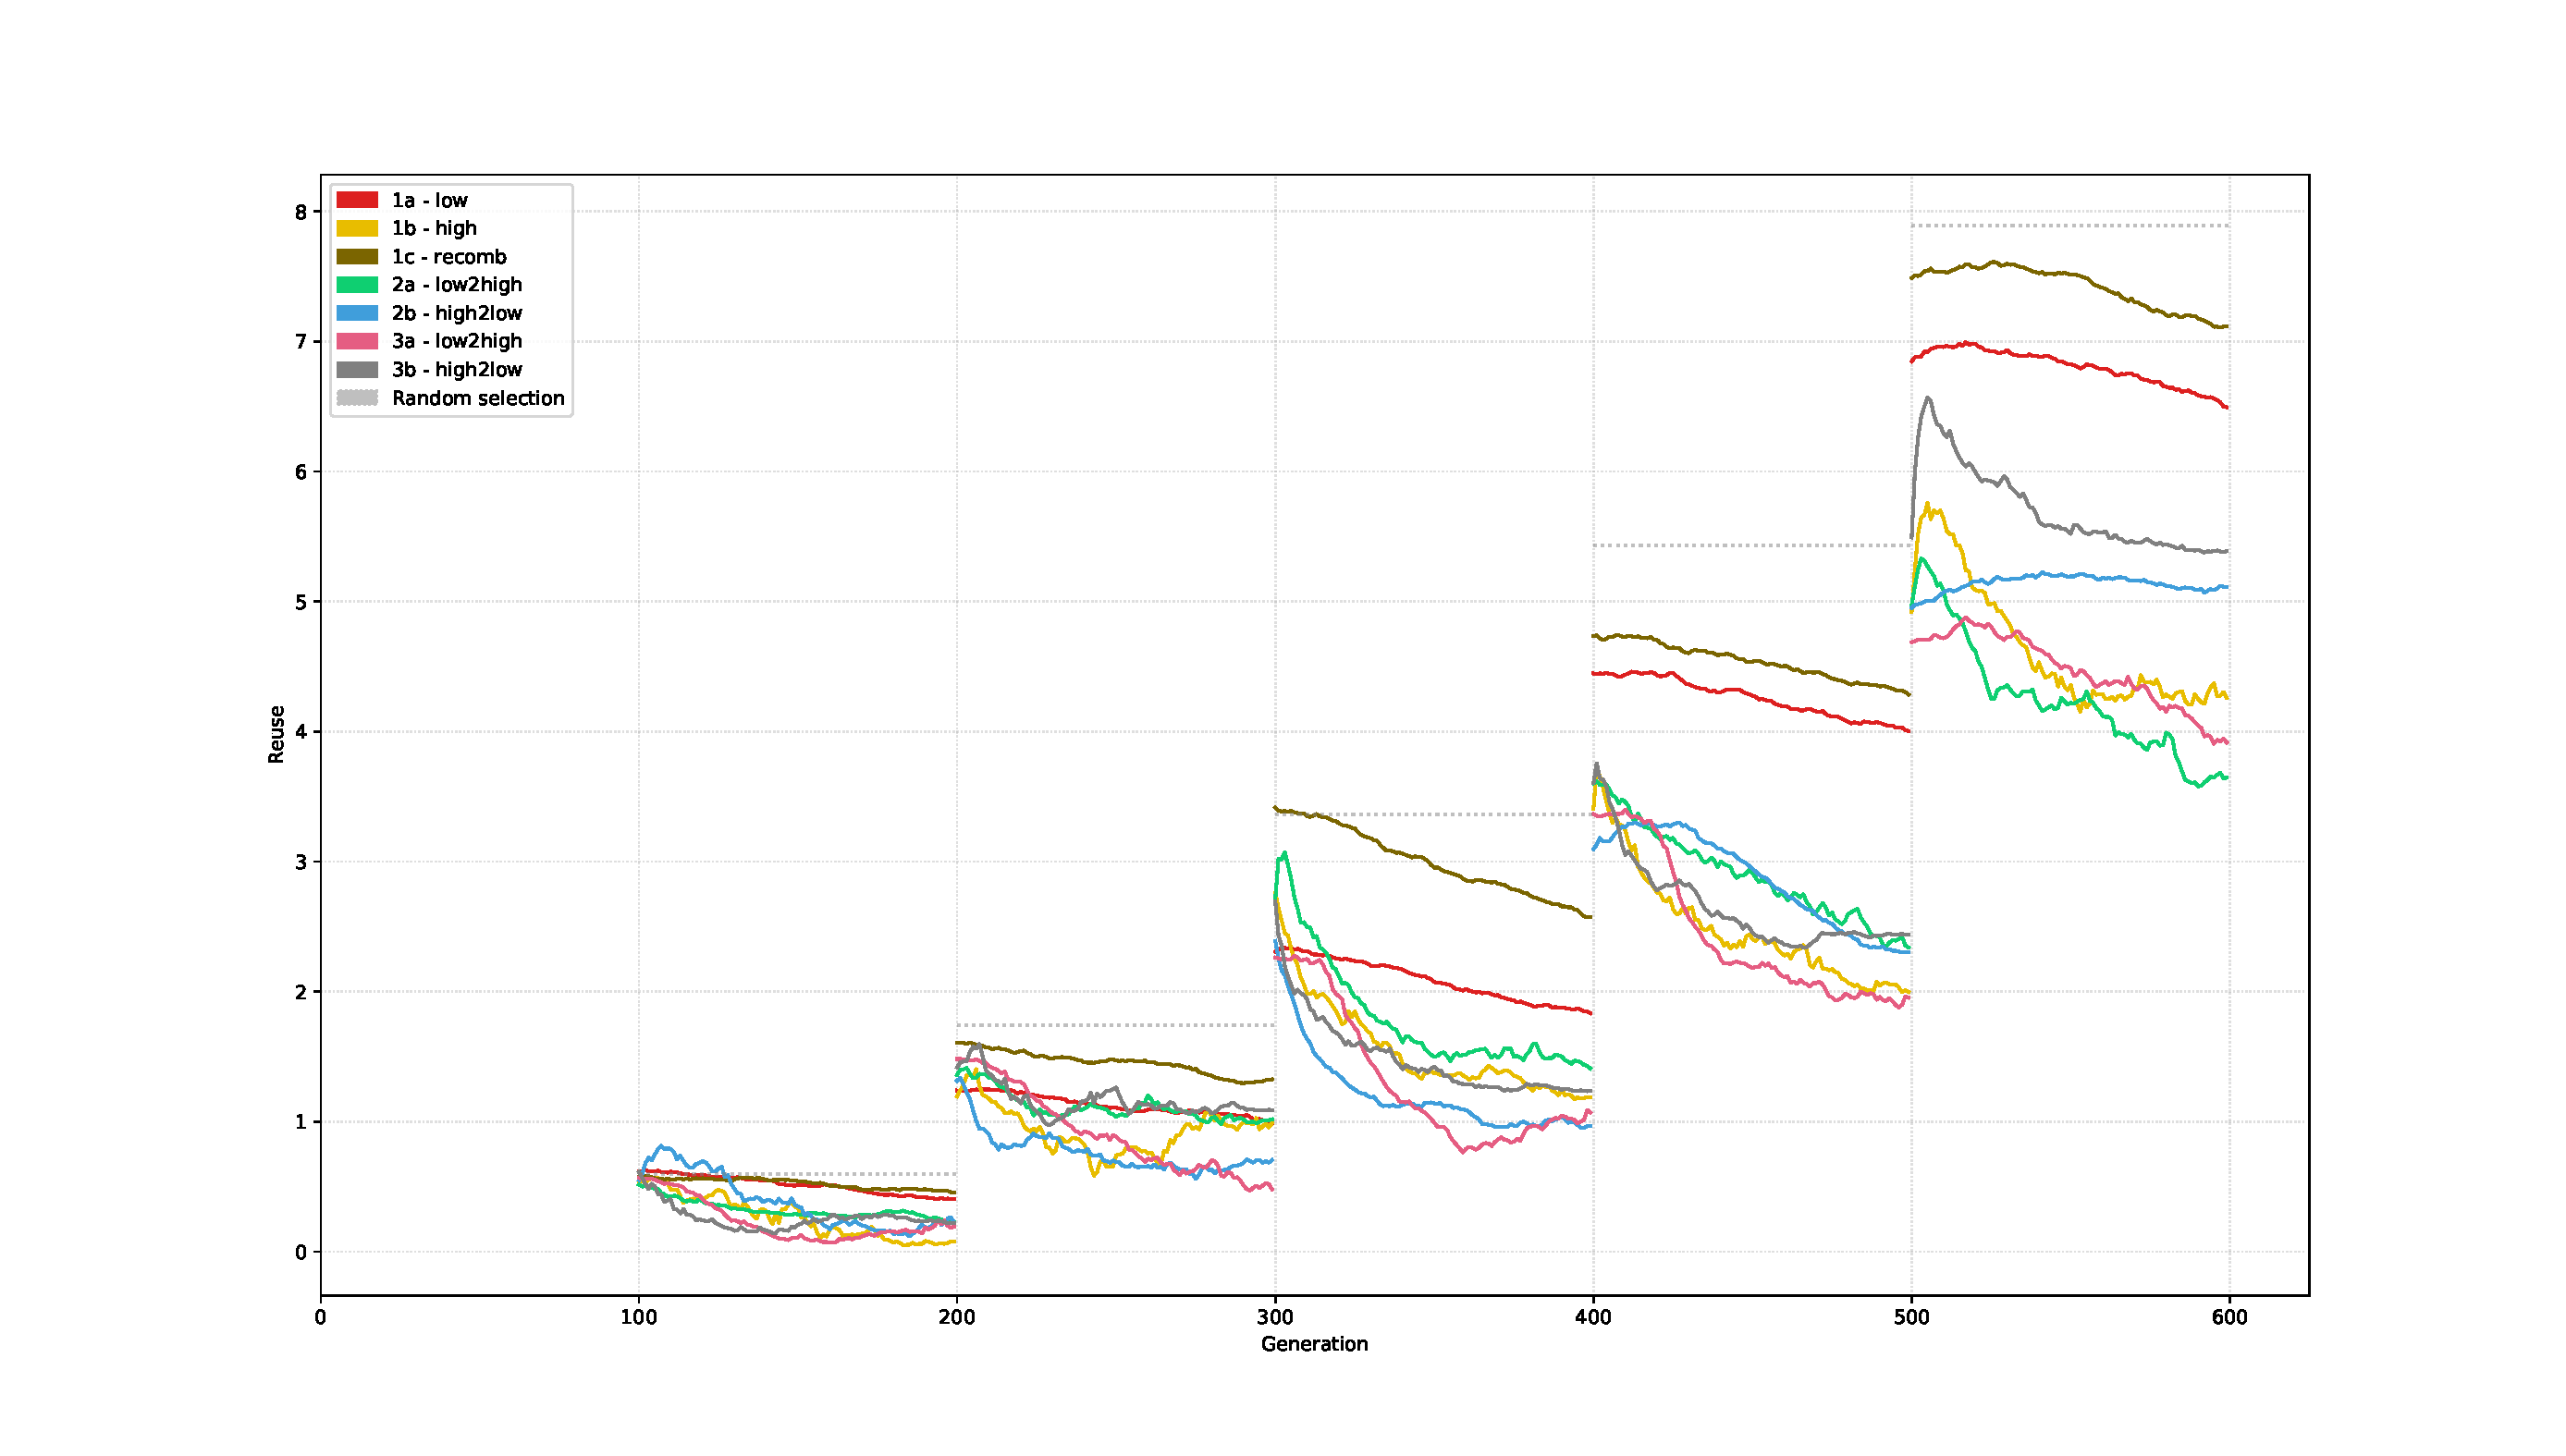
\includegraphics[width=1.2\textwidth,center]{Chapters/4.Experiments/exp2/figures/large/Module_reuse_pr_generation.pdf}
    \caption[Module reuse plot]{The average module reuse during the multi-task learning sequence. Each jump is caused by the saving of an optimal path, and the next task having more locked modules to reuse. The first 100 generations do not have any previously learned knowledge to reuse.}
    \label{fig:search.reuse}
\end{sidewaysfigure}

Comparing the algorithms total usage of the PathNet through the capacity-metric with MWW-tests provided no significant differences. Figure \ref{fig:search.reuse} on the other hand contain escalating fluctuations in the mean reuse across each algorithm. While all are below the Monte-Carlo estimated reuse, the algorithms seem to affect the change in reuse within each search differently. Another round of MWW tests, however, disproves this (see table \ref{tab:exp2.reuseptable}) as no null-hypotheses could be rejected under the Bonferroni corrected \(\alpha\)-level.

\subsection{Discussion}
While figure \ref{fig:search.reuse} show some differences, the results from these experiments seem to conclude that different tournament sizes do not have any effect on the reuse of modules. The results seen here might be different for other tasks, however, as a large difference in task difficulty could cause a PathNet with too little capacity to behave differently.

The Monte-Carlo estimation of reuse and capacity use was run for \(10^{6}\) trials, making the estimated value accurate to 4 decimal places if holding to a MSE 1 order of magnitude less than estimates (see formula \ref{eq:montecarloP}). It is noteworthy that the MWW-tests shows all algorithms being equal, but all algorithms performing significantly different from the Mote-Carlo estimates. 

This shows that the search actively select untrained modules, but also tat we might be seeing something similar to experiment in chapter \ref{exp1}, where the tasks were simple enough for modules to optimize quicker to training data than to the interface of trained modules.

\section{Population diversity}
\label{exp2:diversity}
\subsection{Results}
\ref{fig:search.hamming_diversity} visualizes the average population diversity for each algorithm for each task calculated with the pair-wise Hamming distance metric. 

\begin{sidewaysfigure}[p!]
    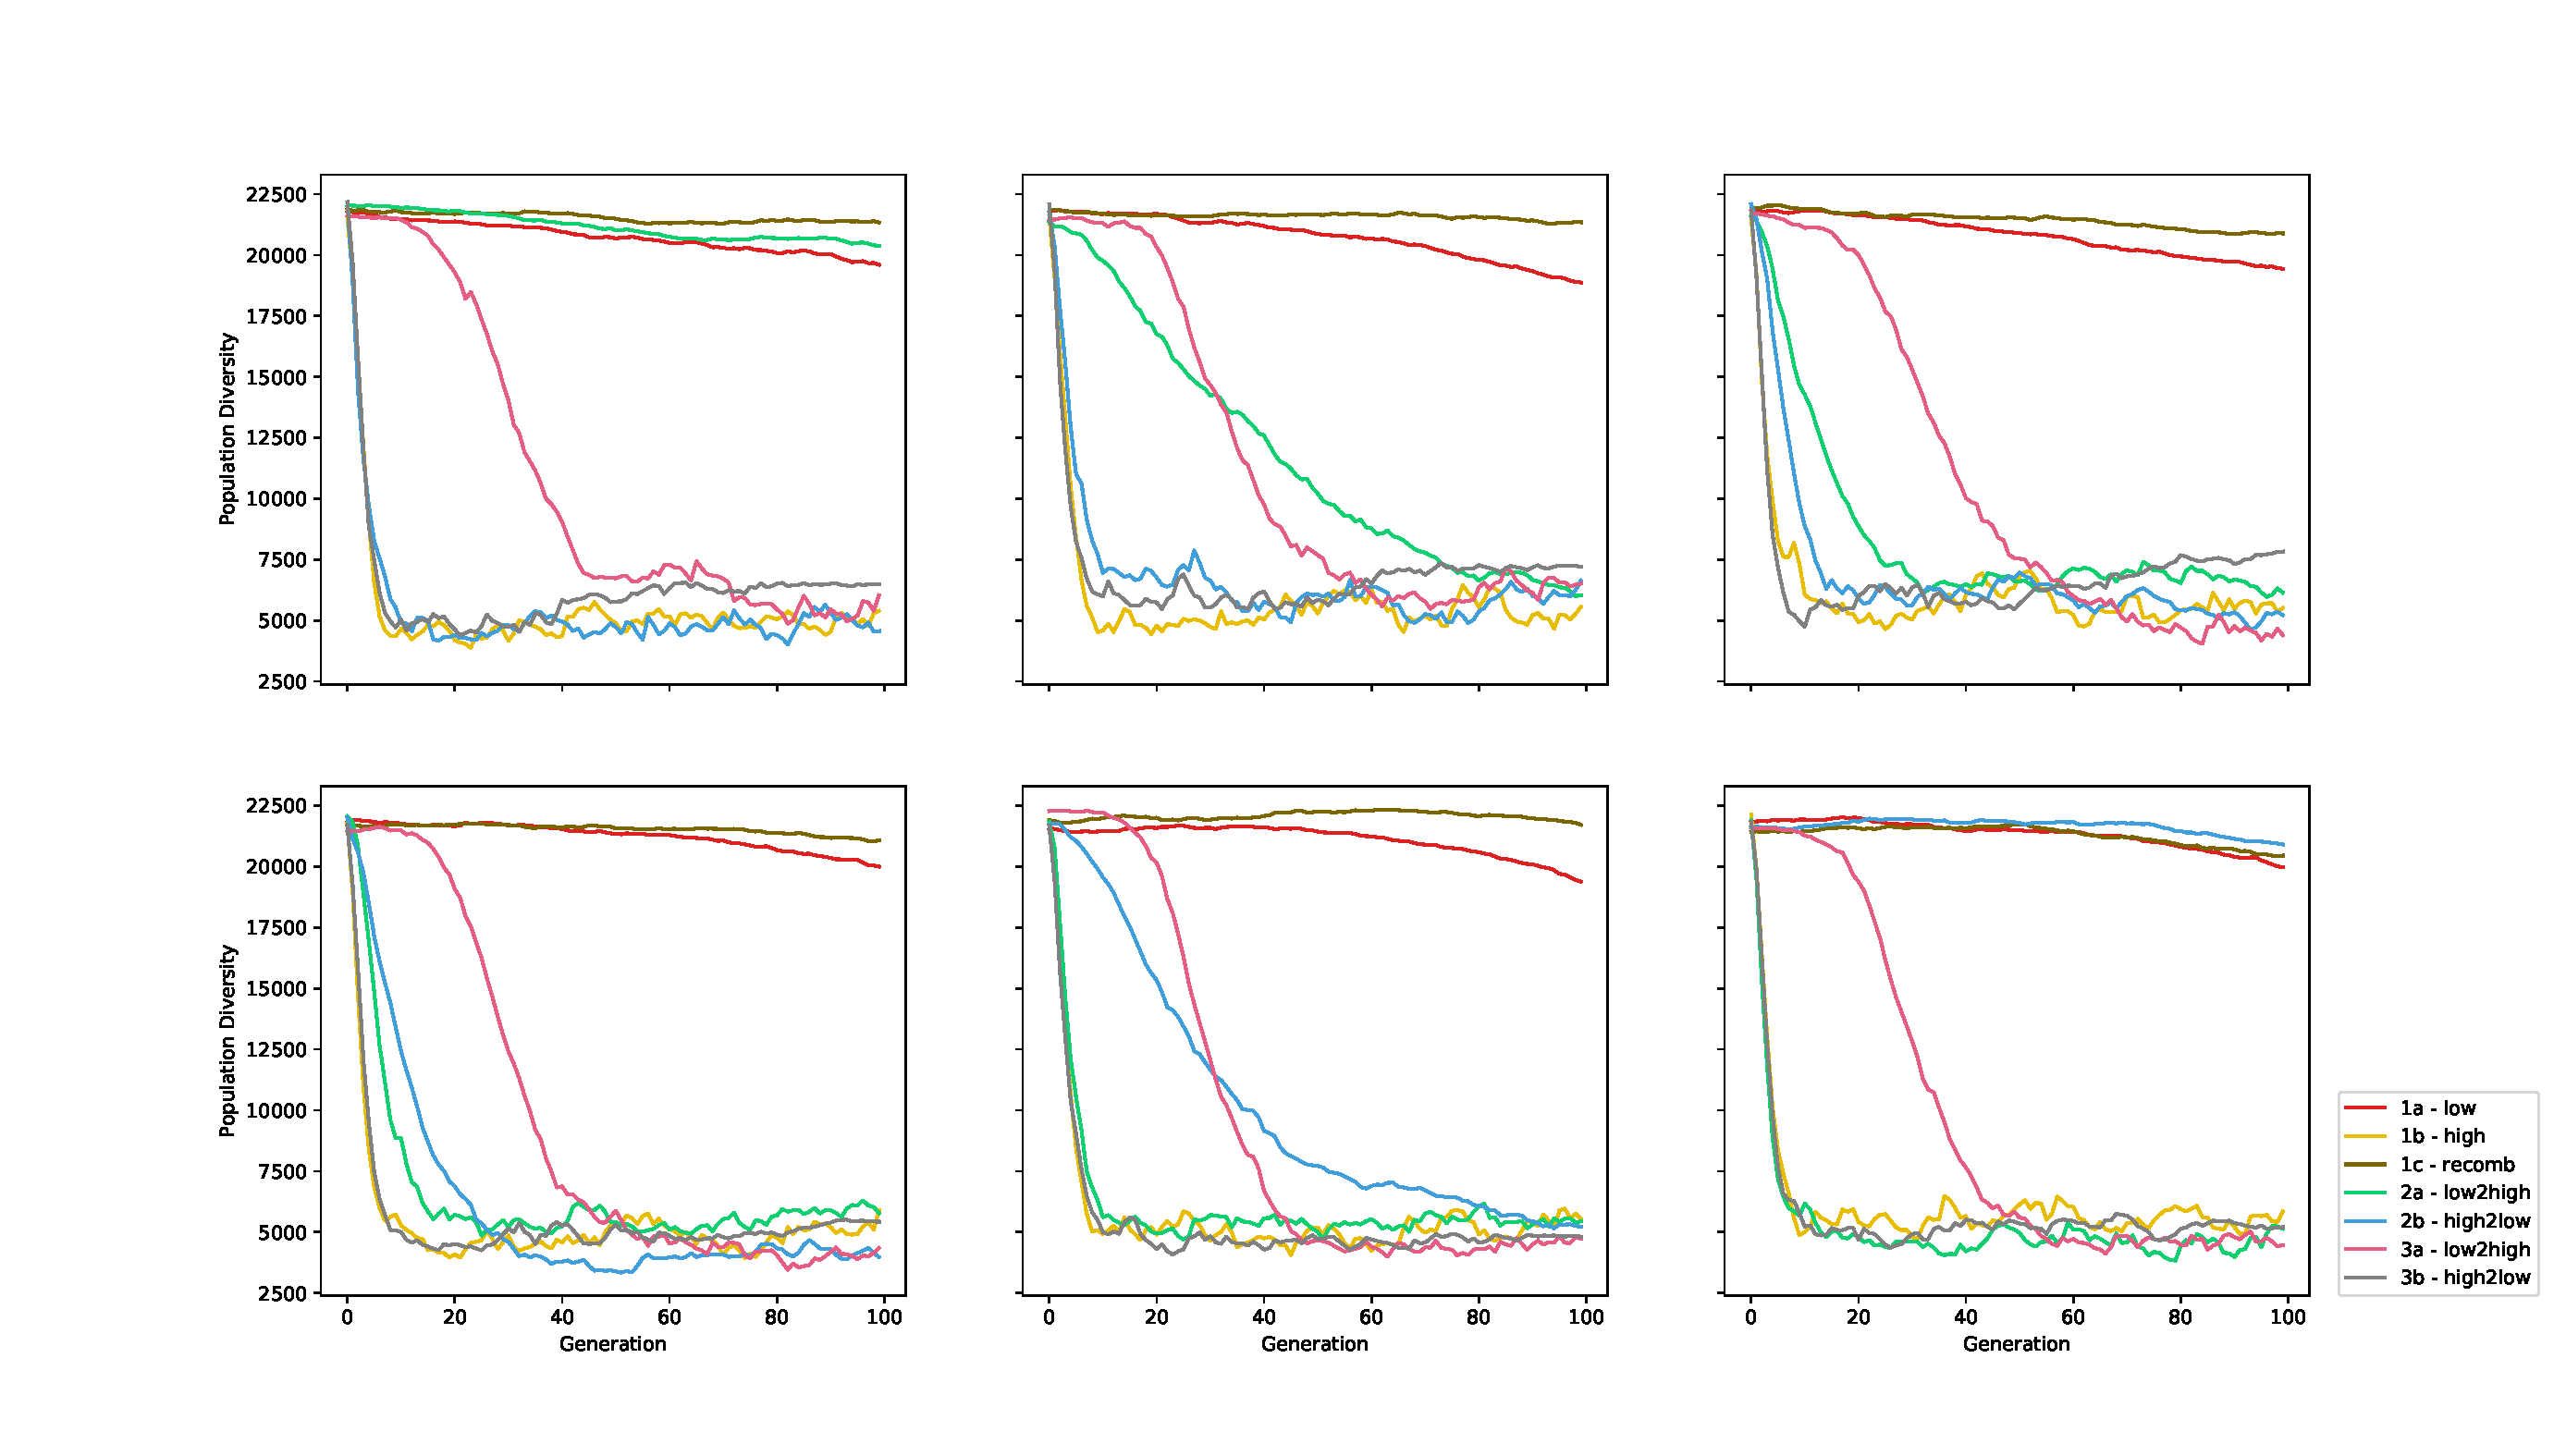
\includegraphics[width=1.2\textwidth,center]{Chapters/4.Experiments/exp2/figures/large/Average_population_diversity_reduced_hamming.pdf}
    \caption[Pair-wise Hamming distance diversity]{The average pairwise Hamming distance within each generation is used as a measure for population diversity. Each subplot (in order left to right) is each task in trained order.}
    \label{fig:search.hamming_diversity}
\end{sidewaysfigure}

When a generation is over, and mutations of the tournament winner replace all losers, the population makes a large shift in diversity unless most of the tournament participants have a similar genome, at which point population has most likely converged. This is why all diversity plots (\ref{fig:search.hamming_diversity} and \ref{fig:search.frequency_diversity_unique}) contain rapid changes for sections of high tournament size, while algorithms 1a and 1c (also algorithm 2a for the first tasks, 2b for the later tasks) have more gradual changes. 

\begin{sidewaysfigure}[p!]
    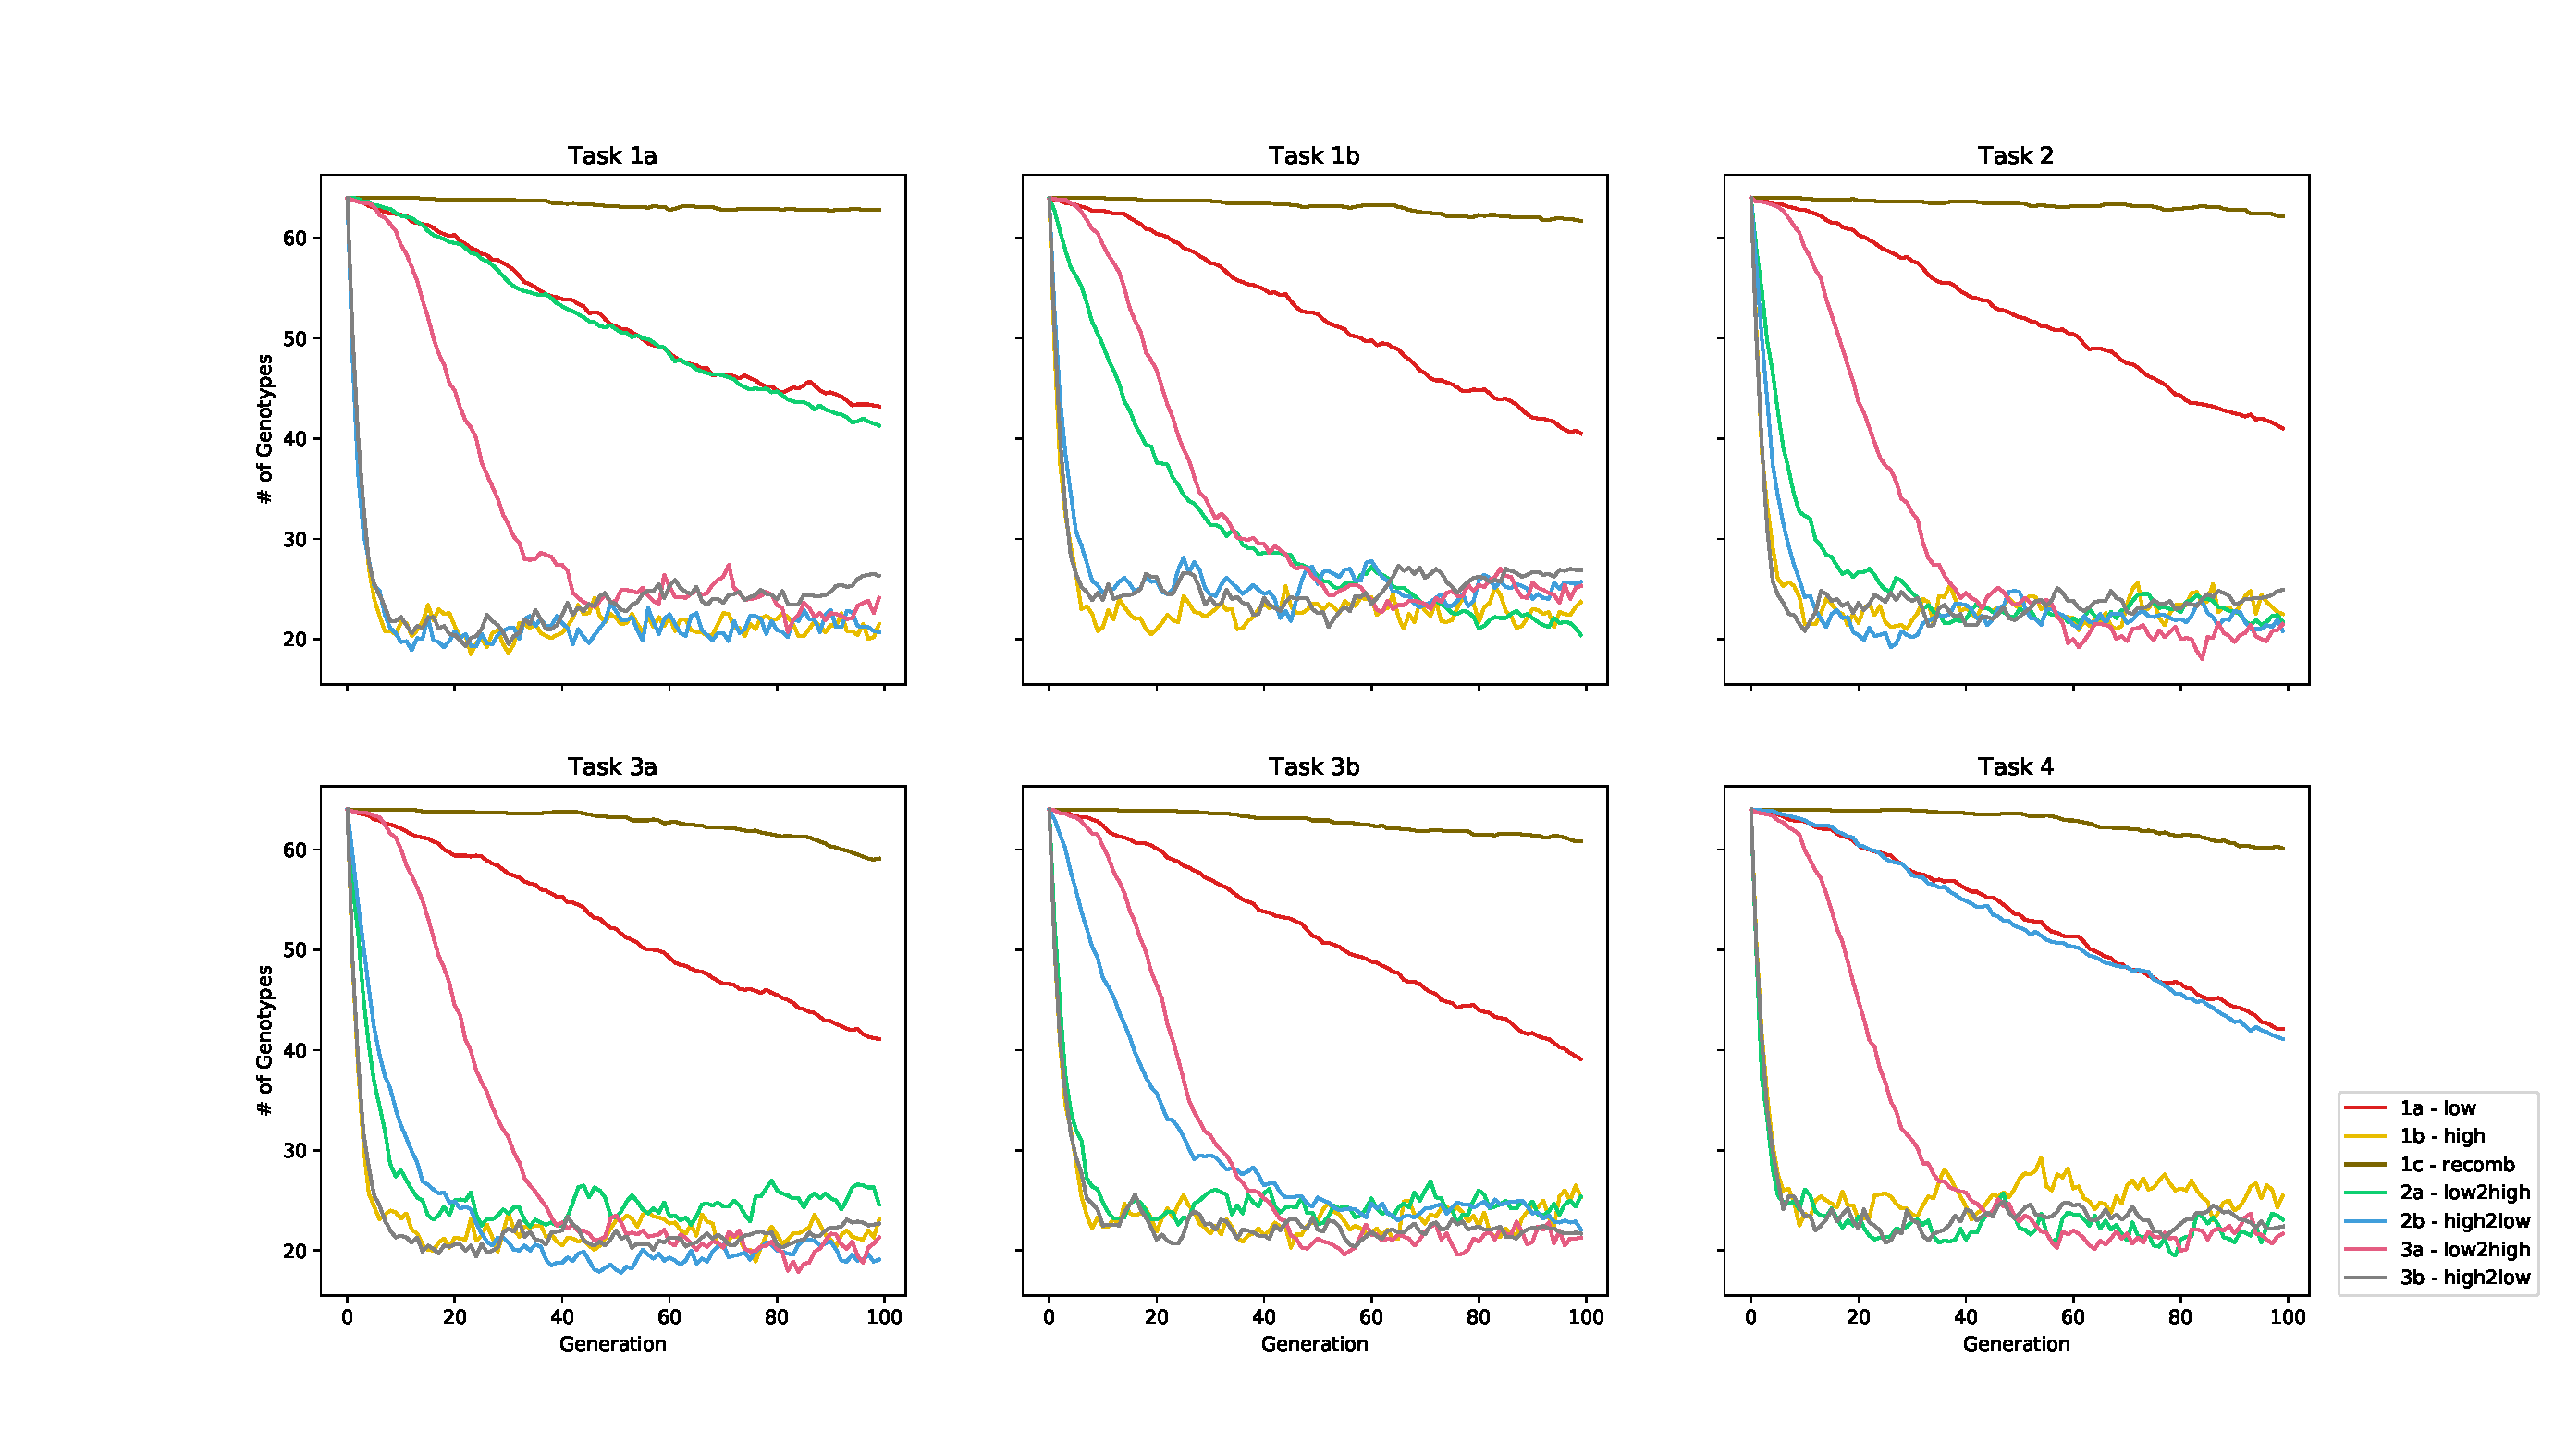
\includegraphics[width=1.2\textwidth,center]{Chapters/4.Experiments/exp2/figures/large/frequency_diversity_unique_path_count.pdf}
    \caption[Unique genome frequency diversity]{The number of unique paths within a population. Plotted for every task and every algorithm.}
    \label{fig:search.frequency_diversity_unique}
\end{sidewaysfigure}

Plots \ref{fig:search.hamming_diversity} and \ref{fig:search.frequency_diversity_unique} contain about the same information, and confirms the ordering of selection pressure is what was intended. The only difference worth mentioning is the one of algorithm 1a for the two plots. We would expect the frequency diversity to misrepresent tie diversity of a population as being higher than it actually is due to it counting small mutations as totally different genomes. Here we see frequency giving a smaller diversity than Hamming distance, which suggests Hamming distance is the one misrepresenting reality. 

Also, note algorithms 2a and 2b. The convergence rate of these algorithms changes as the tournament size does. Comparing these to algorithms 1a and 1b uncovers that tournament size 15, 20 and 25 have no notable difference in convergence rate to algorithms 1b, while there is a small but visible difference for tournament size 10. Size 5 is the only one distinguishing itself from other tournament sizes or selection pressure schemes. 

Grouping by convergence rate would indicate tournament sizes 10, 15, 20 and 25 are equal to each other and algorithm 3b. 3a is much the same as tournament size 5. 1a is slow but steadily converging and would most likely do so if the generation termination limit was increased, while 1c shows no such tendencies. 

\subsection{Discussion}
As hypothesized, low tournament size yielded low convergence rate while high tournament size gave high convergence. Figures \ref{fig:search.hamming_diversity} and \ref{fig:search.frequency_diversity_unique} also makes it possible to rank the algorithms by its selection pressure on a \textit{"exploration vs. exploitation"} scale. Algorithms 2a and 2b change throughout the multi-task scenario, and their selection pressure follow this change. Algorithms 3a and 3b, however, behave the same for each path-search. From the plots, it is obvious that algorithm 3a has a lower convergence rate than 3b, as its tournament size starts out small and grows during the search. I.e., algorithm 3a has a lower selection pressure than algorithm 3b. 

Looking at algorithms 2a and 2b in figures \ref{fig:search.hamming_diversity} and \ref{fig:search.frequency_diversity_unique}, it seems the tournament size does not scale linearly with convergence. Tournament sizes 10, 15, 20 and 25 have similar convergence rate to that of algorithm 1b. This would indicate that a static tournament size of 10 would provide similar exploration and exploitation to a path search as a tournament size of 25. 

While both algorithm 1a and 1c have low selection pressure and therefore also a low convergence rate, figure \ref{fig:search.frequency_diversity_unique} has a notably inadequate description of the diversity of algorithm 1c. The recombination functionality ensures the offspring of two genomes are genetically different from both parents even though the overall genetic diversity has dropped.

\section{Training}

\subsection{Results}

\begin{sidewaysfigure}[p!]
    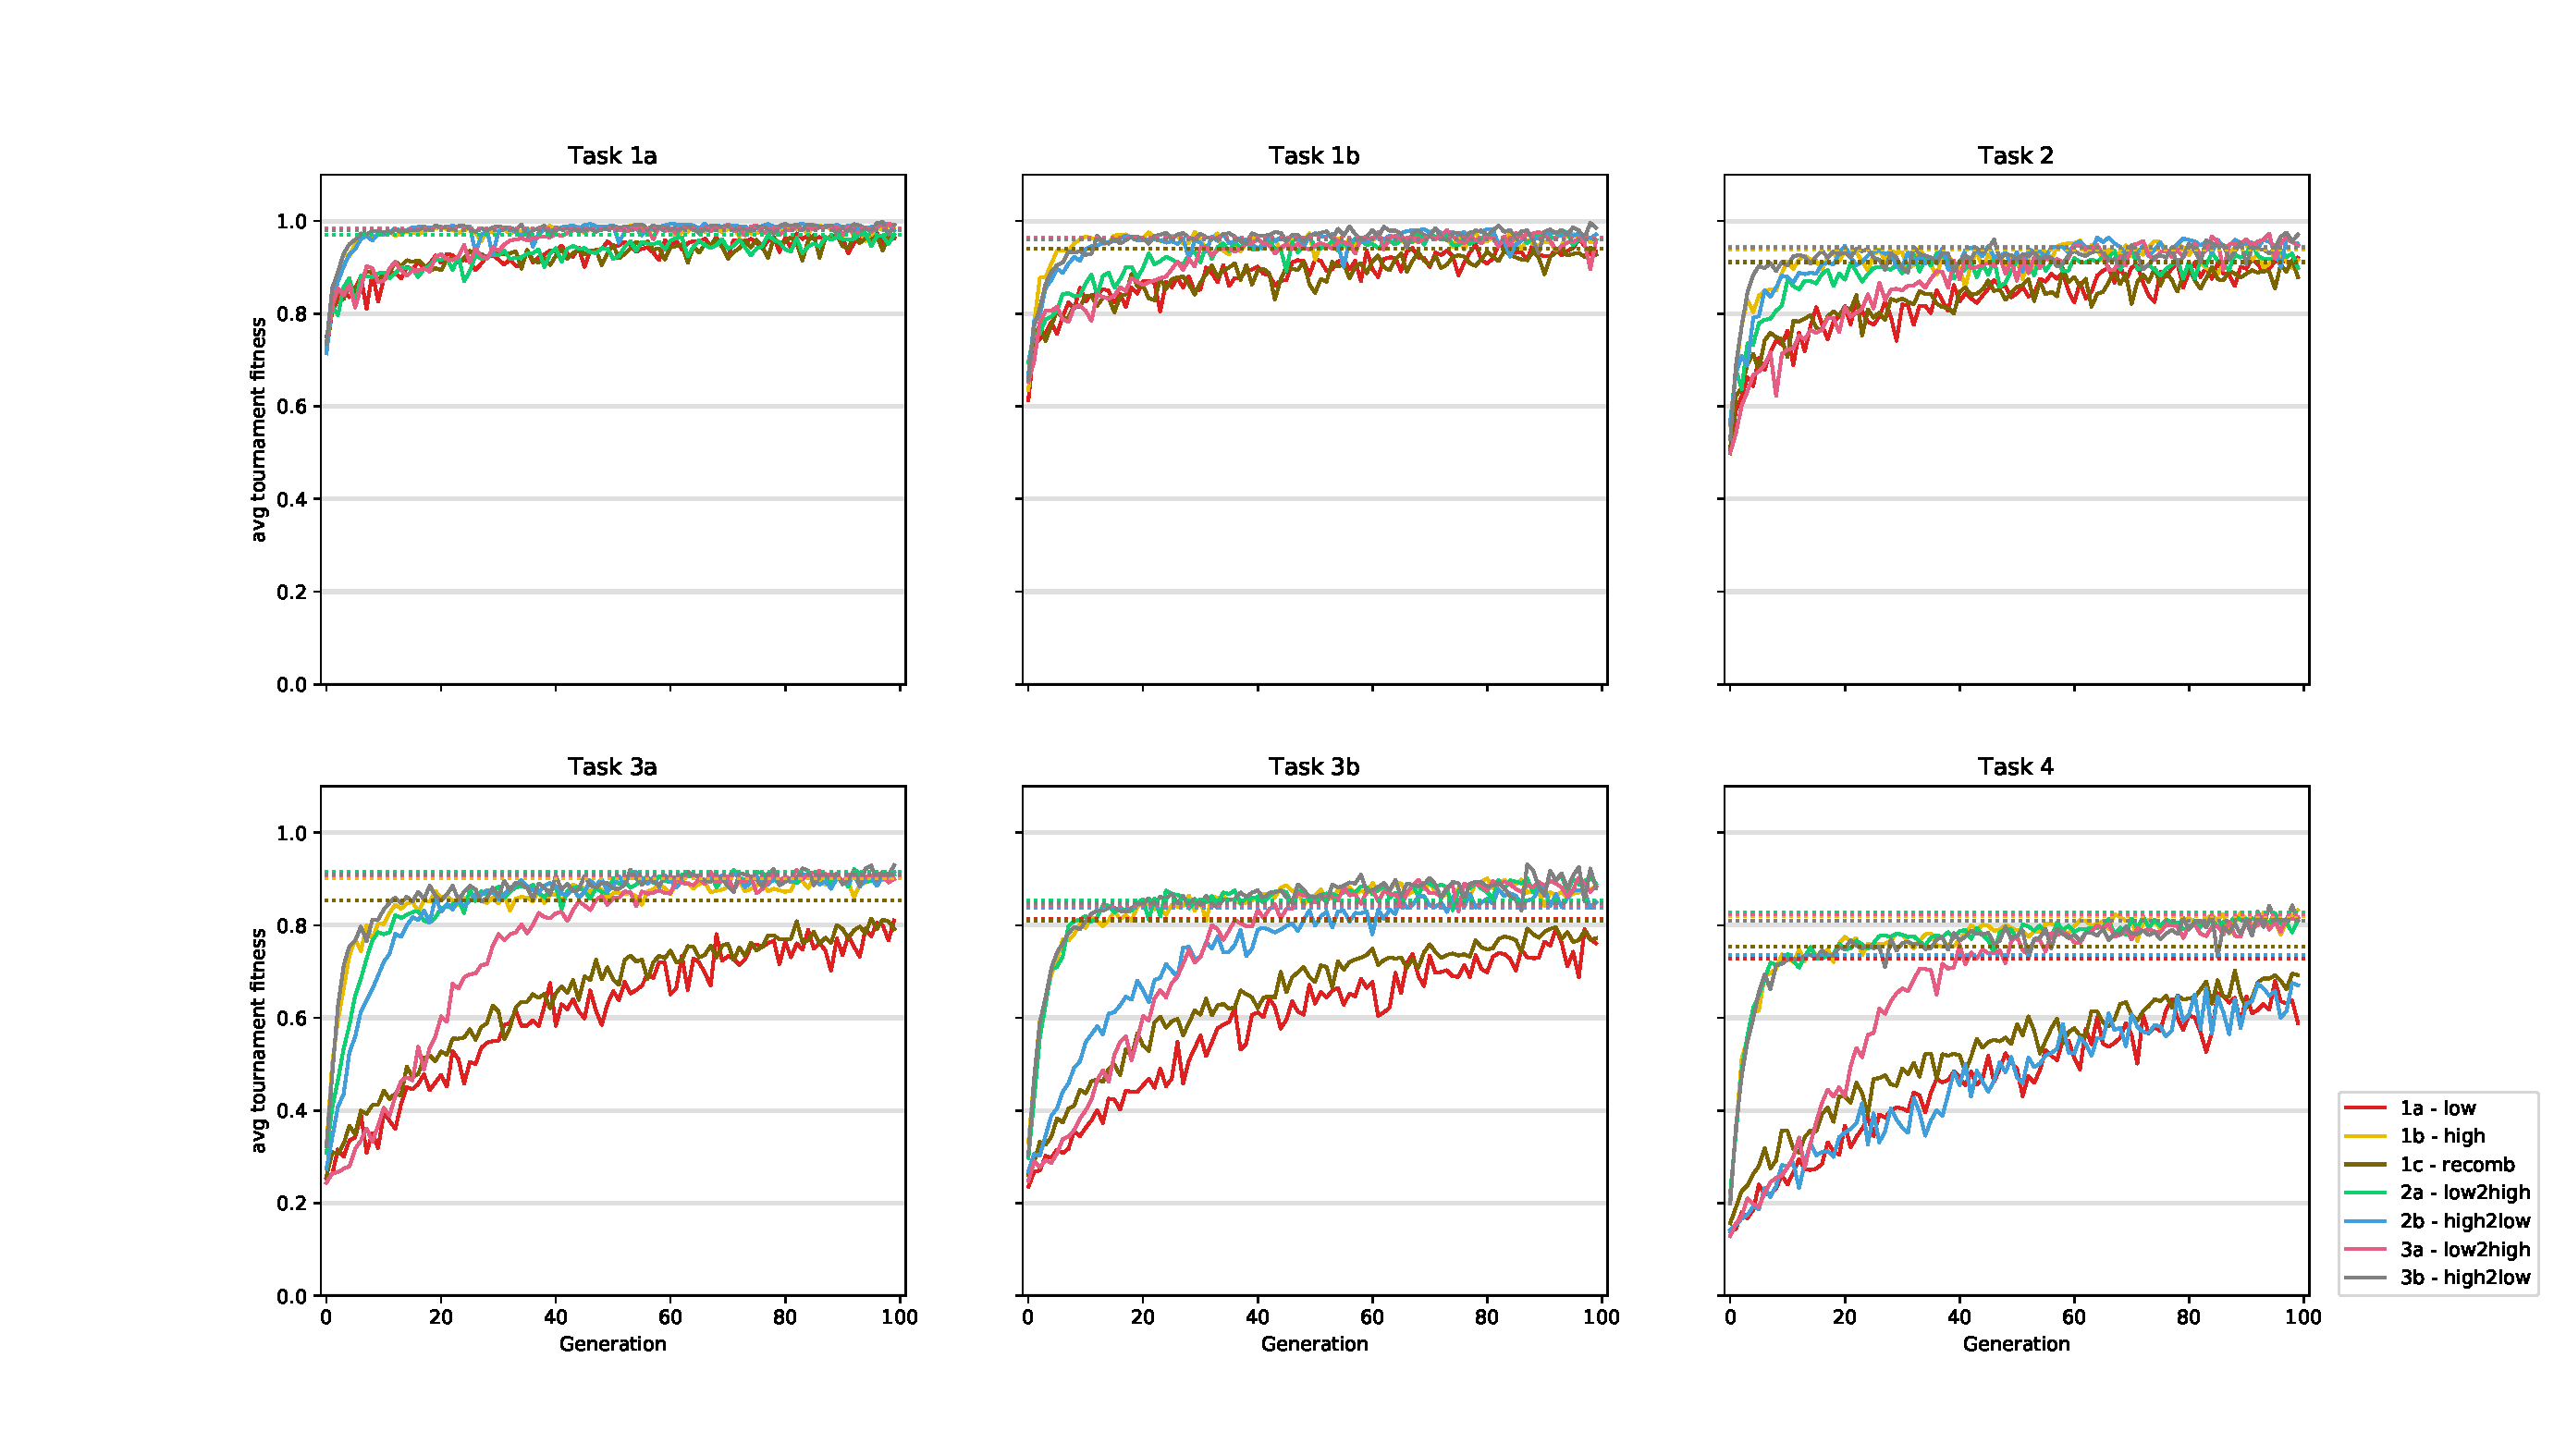
\includegraphics[width=1.2\textwidth,center]{Chapters/4.Experiments/exp2/figures/large/Training_accuracy.pdf}
    \caption[Fitness plot]{Average fitness during search. The dotted lines is the average achieved validation accuracy for that task and that algorithm.}
    \label{fig:search.accuracy}
\end{sidewaysfigure}

As the training of each path is done during and controlled by the search, how the average training accuracy develops gives an indication of how quickly the algorithms are able to influence the overall PathNet to learn a task. As discussed in section \ref{exp2:implementation.search}, the act of training one tournament of genomes affect the previously evaluated fitness values. Because of this, the populations average fitness value would be a highly misleading metric to use and therefore what is plotted in figure \ref{fig:search.accuracy} is the average fitness score achieved within each generations tournament. Also plotted is the mean validation accuracy reached for each algorithm. This validation score is only calculated after an optimal path have been found for each task, and can therefore not be viewed as a function of generation number. The validation accuracy is visualized separately as a box-plot in figure \ref{fig:search.validation}.

\begin{sidewaysfigure}[p!]
    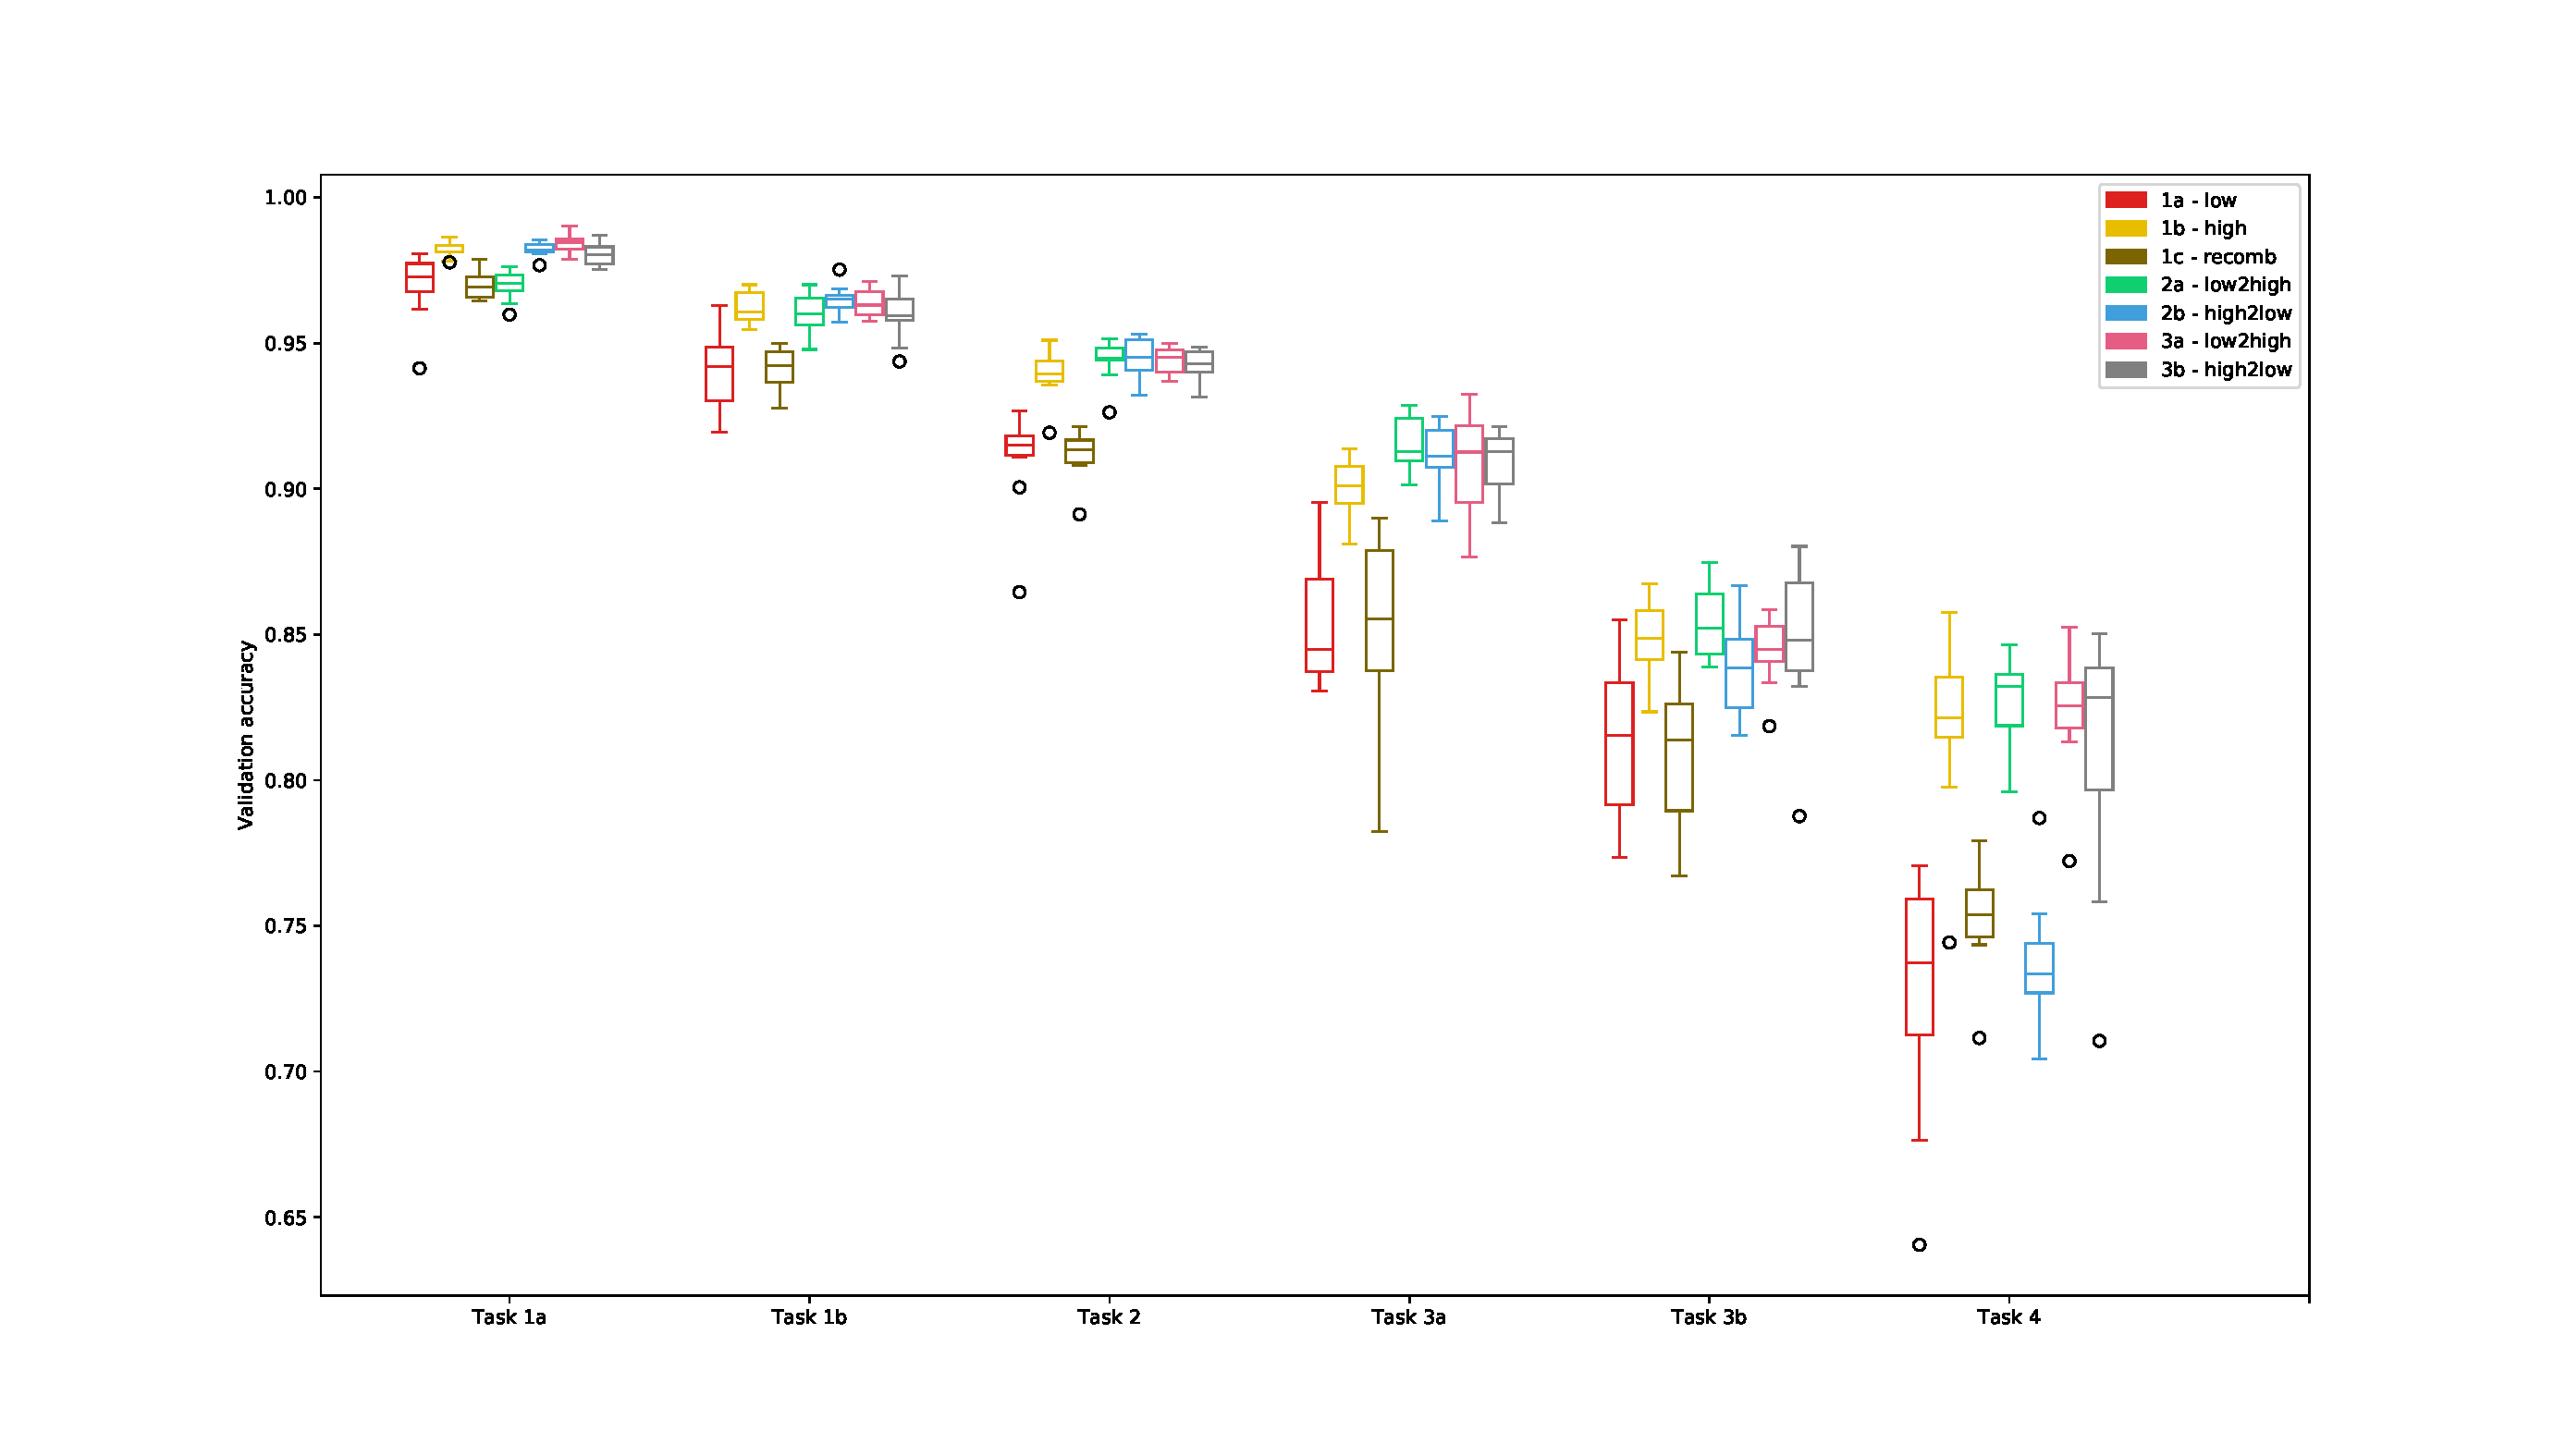
\includegraphics[width=1.2\textwidth, center]{Chapters/4.Experiments/exp2/figures/large/validation_boxplot.pdf}
    \caption[Validation accuracy plot]{Boxplot of validation accuracy reached for each task and each algorithm.}
    \label{fig:search.validation}
\end{sidewaysfigure}

Again, one MWW-test is run for every pair of algorithm for each task, this time to test the distributions of validation accuracies under the \(\alpha\)-level 0.0003968. Comparing this \(\alpha\) to results in tables in section \ref{appendix:ptable.accuracy}, some patterns emerge: 
\begin{itemize}
    \item Low tournament size: There is no significant difference in accuracy distribution between the algorithms with static low tournament size. The algorithms 2a and 2b are also similar to 1a and 1c for those tasks where they have a low tournament size. Meaning task 1a for algorithm 2a and task 3b and 4 for algorithm 2b. 
    \item High tournament size: Algorithm 1b is only significantly different from other algorithms when they use a tournament size of 2 or 3, the exception being algorithm 1a for task 3b and 4, where the null-hypothesis cannot be rejected. 
    \item Changing tournament size: Algorithms 2a and 2b differ significantly only when their tournament size is most different; tasks 1a and 4. 
    \item Dynamic tournament size: Algorithms 3a and 3b does not differ for any task, and are also similar to algorithm 1b for all tasks. They do seem to differ from the low tournament size algorithms for most tasks, however, except task 3b. 
\end{itemize}

\begin{sidewaysfigure}[p!]
    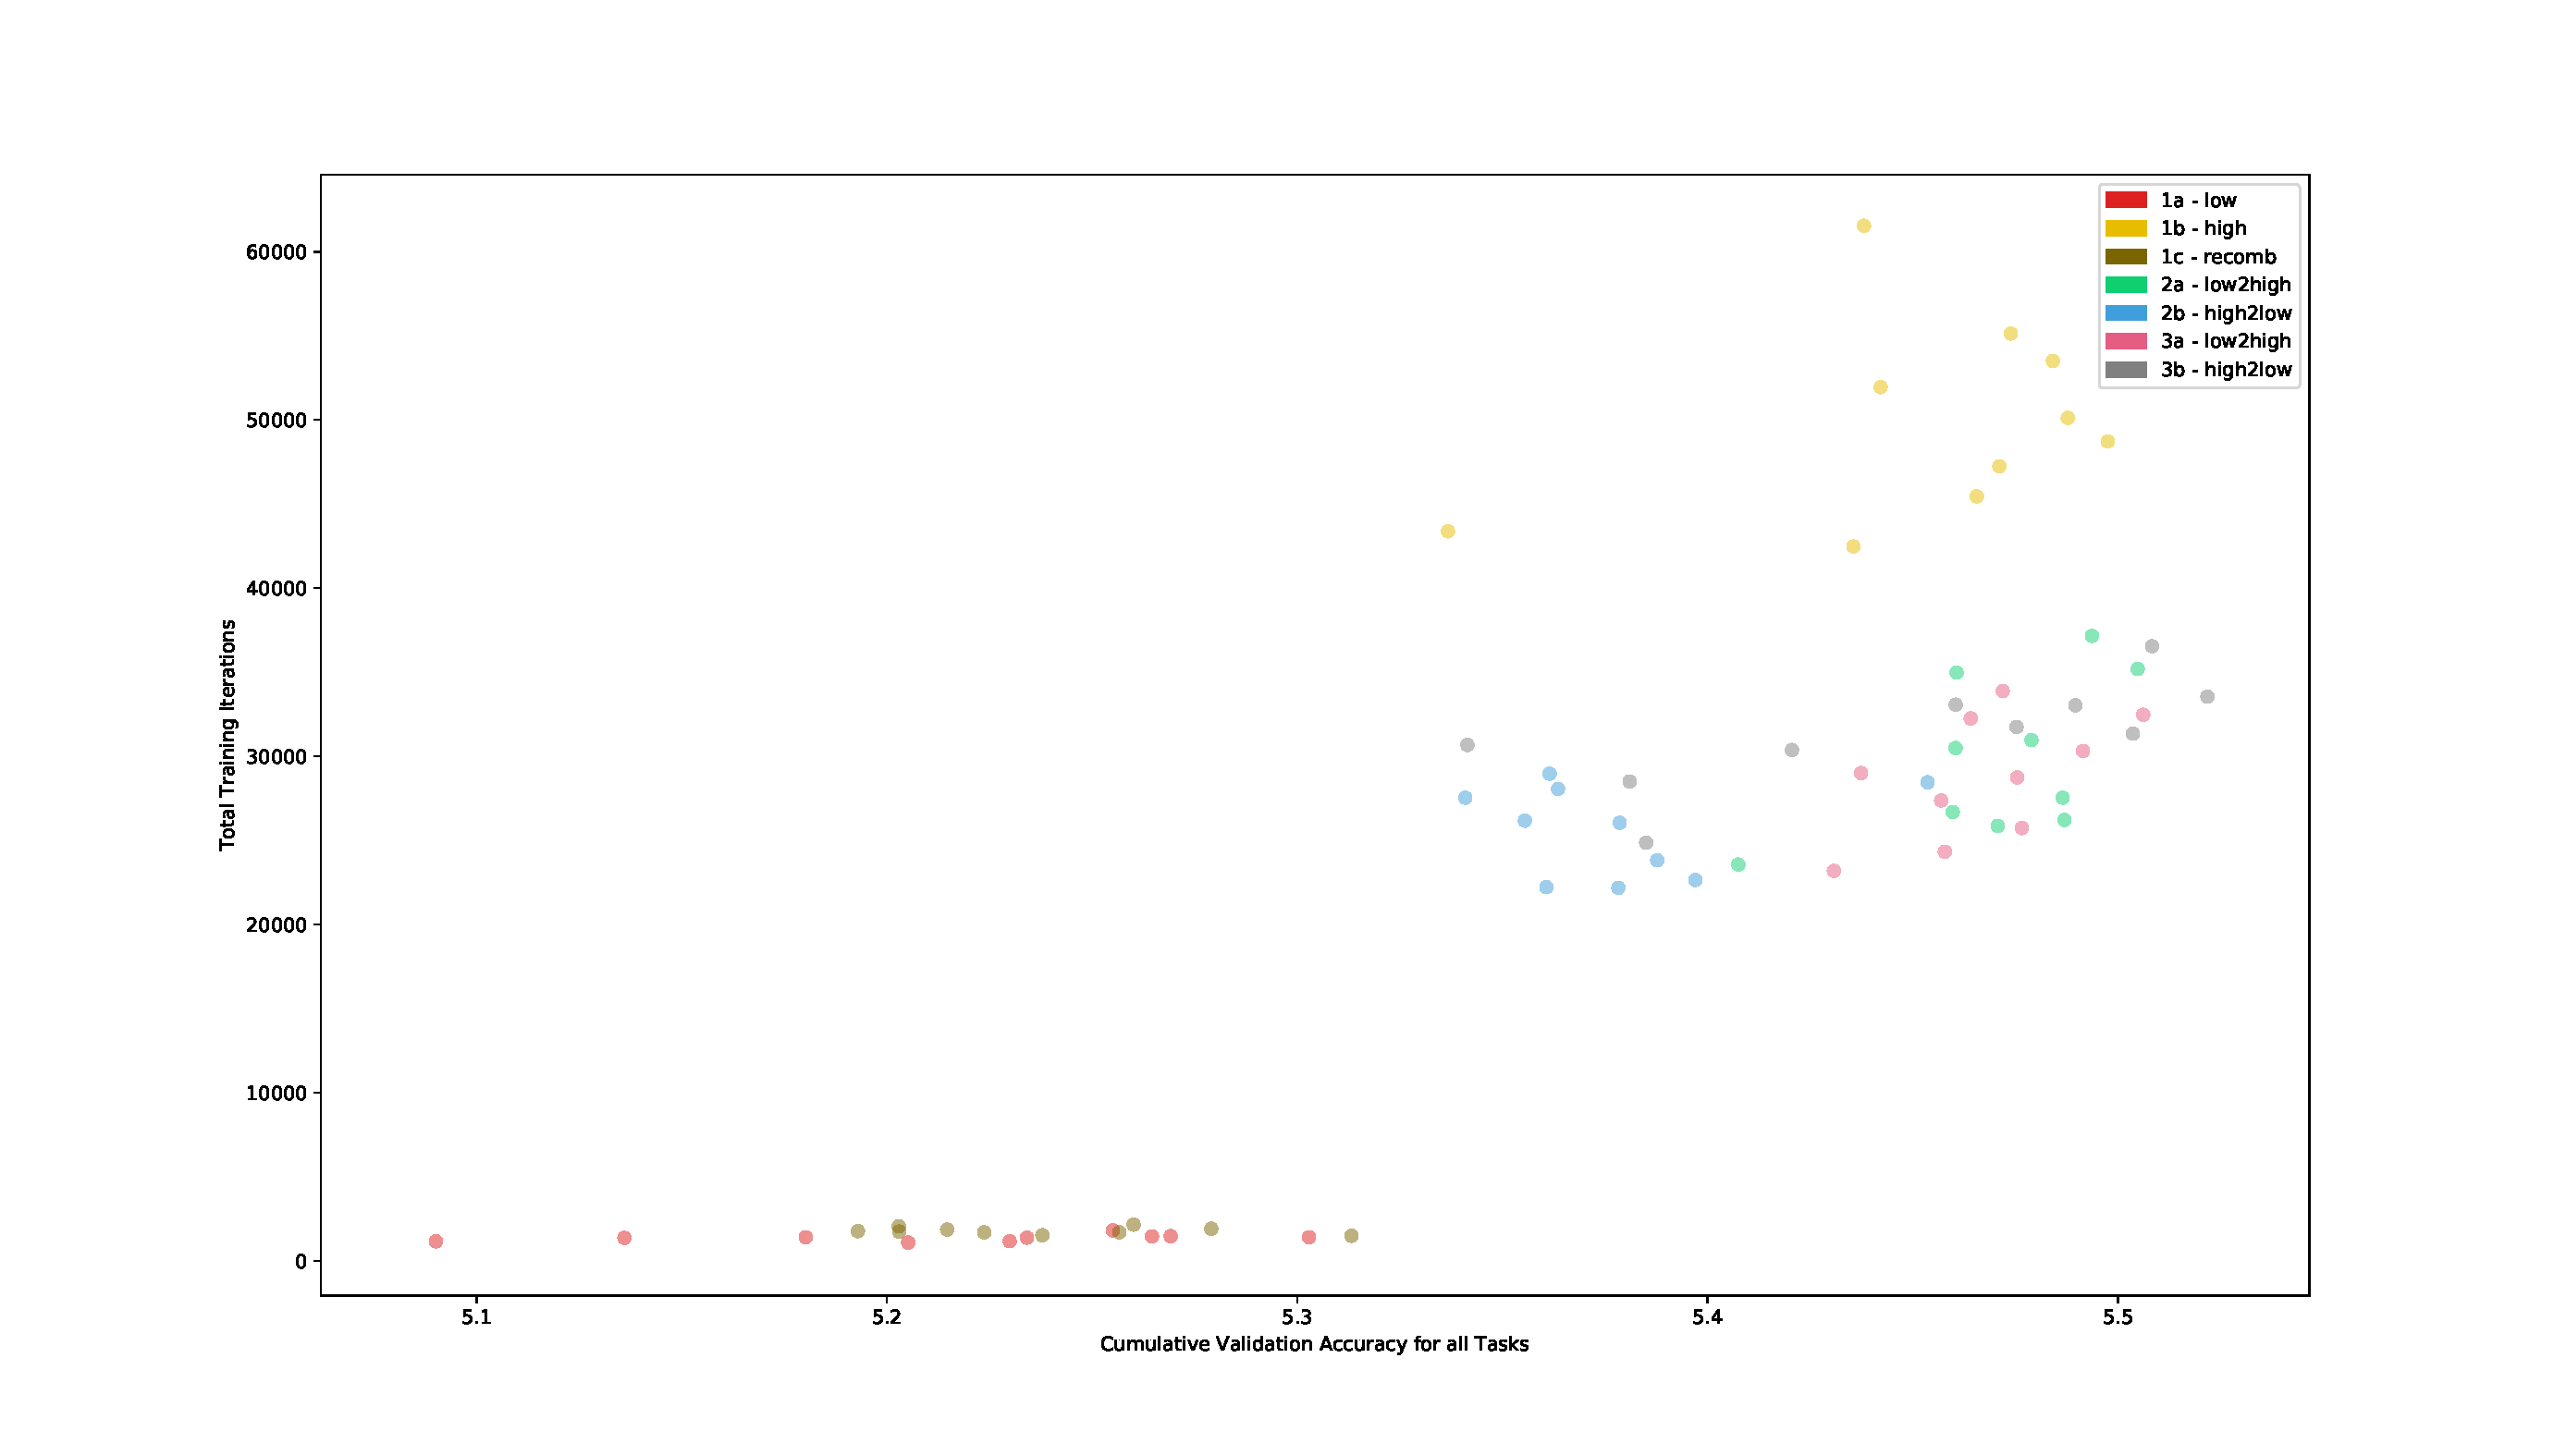
\includegraphics[width=1.2\textwidth,center]{Chapters/4.Experiments/exp2/figures/large/Training_value.pdf}
    \caption[Training vs cumulative accuracy plot]{The total amount of training in all optimal paths for each multi-task learning sequence plotted against the cumulative validation accuracy reached for that sequence. The circle size corresponds to the total number of used PathNet modules.}
    \label{fig:search.training_value}
\end{sidewaysfigure}

Training value figure \ref{fig:search.training_value} shows us much of the same as \ref{fig:search.validation}, the difference being the x-axis is the cumulative accuracy reached for all six tasks and the y-axis shows the total amount of training units for all optimal paths found. The circle radius for each trial is correlated to the total use of modules. 

The similarity in performance for algorithms 1a and 1c is present here also, as well as the similarity in validation accuracy for algorithms 1b, 2a, 2b, 3a, and 3b. These are separated in training amount, however, which is not surprising as this is highly correlated to the tournament size and this changes between the algorithms. The difference in cumulative accuracy between task 2a and 2b seem to be about 0.1, and can, therefore, be explained by solely by the difference in validation accuracy between these two algorithms for task 4 as seen in figure \ref{fig:search.validation}. The small tournament size of 2 in algorithms 2b yields a accuracy around ten percentage points lower than 2a for this task, giving 2b a lower cumulative score in figure \ref{fig:search.training_value}. Tournament size 2 is still enough to reach a high performance for task 1a, which means this inequality is not equalized when 2a use a low tournament size. 

MWW testing of training amounts does not introduce something not found in plot \ref{fig:search.training_value}. Algorithms 1a, 1b, and 1c are significantly different from all other algorithms, including each other. Within the cluster of algorithms 2a, 2b, 3a, and 3b, the only pair that differs are 2a and 3b. 

\subsection{Discussion}
For the three first tasks 1a, 1b and 2 (all based on MNIST) figure \ref{fig:search.accuracy} the tasks are too simple for the algorithms to show any difference as any selection pressure used is capable of reaching a high performance for these tasks. For those based on cSVHN however, a clear split is visible for the algorithms. The split seem to follow the same pattern as the diversity plots \ref{fig:search.hamming_diversity} and \ref{fig:search.frequency_diversity_unique}. The low selection pressure algorithms are steadily increasing in fitness throughout the search, and the fitness is still improving when the search terminates, hinting at 100 generations being too little for these algorithms to reach the same performance as those of higher tournament sizes. This is what was hypothesized and is explained by the increase in evaluations (and therefore also training units) for algorithms with higher tournament sizes. The similar fitness progression of 2a and 2b when using tournament size of 10 and higher to that of algorithms 1b, 3a and 3b are interesting, however. This points towards the performance of tournament size above ten not being different. Figure \ref{fig:search.validation} supports this suspicions. The MWW-tests for these results are indeed statistically significant.

When setting this accuracy in the context of training in figure \ref{fig:search.training_value} it becomes clear the maximum tournament size of 25 is set unnecessarily high. A static use of tournament size around ten would yield a similar accuracy performance to that of algorithms 1b, 2a, 2b, 3a, and 3b while having a significantly lower training amount than any of these.

\section{Tournament size range}
For these experiments, the results show that using a tournament size above ten is unnecessary. Under this assumption, algorithms 3a and 3b would more than likely perform differently as their increase in selection pressure were intended to be more or less linear, while it here reaches the top level of selection pressure within the first 40\% of each search. 

As the plot \ref{fig:search.accuracy} show, the algorithms with high tournament size reach their maximum fitness quite early in the search. The remaining 60\% of search time\footnote{During the last 60\% of the search, algorithm 3a have functionally the maximum amount of selection pressure. This is also the case for algorithm 3b for the \textit{first} 60\% of the search} should be enough search time to learn each task. I.e., algorithms 3a and 3b effectively function the same as algorithm 1b.

By changing the range of tournament sizes these algorithms use, we would presumably reduce their accuracy performance to be somewhere between that of a constantly high and a constantly low selection pressure.

To verify the change in selection pressure have a effective range from the low tournament size in algorithms 1a, and 1c and to tournament size 10, algorithms 3a and 3b are rerun within the range \([2,\dots,10]\). MWW tests provided the results found in table \ref{tab:exp2.dynamic_rerun}, where algorithm 3a with the range 2 through 25 is compared to algorithm 3a with range 2 through 10, and the same comparison made for algorithm 3b. 

\begin{table}[h]
    \centering
    \begin{tabular}{lrrrrrr}
            & \multicolumn{2}{r}{Reuse} & \multicolumn{2}{r}{Accuracy} & \multicolumn{2}{r}{Path size} \\
            & 3a          & 3b          & 3a            & 3b           & 3a            & 3b            \\
    Task 1a &             &             & 0.6771        & 0.0279       & 0.9690        & 0.5593        \\
    Task 1b & 0.9565      & 0.9565      & 0.9397        & 0.4488       & 0.1816        & 0.2366        \\
    Task 2  & 0.5381      & 0.5621      & 0.5966        & 0.6775       & 0.8770        & 0.2440        \\
    Task 3a & 0.6028      & 1.0         & 0.8205        & 0.4272       & 1.0           & 0.8770        \\
    Task 3b & 0.7576      & 0.6969      & 0.6224        & 0.0815       & 0.9057        & 0.0624        \\
    Task 4  & 0.2687      & 0.7837      & 0.0539        & 0.6500       & 0.1361        & 0.3086       
    \end{tabular}
    \caption{P-values from comparing algorithms 3a and 3b for a tournament size range of \([2,\dots,25]\) with range \([2,\dots,10]\). \(\alpha=1.57\times 10^{-3}\)}
    \label{tab:exp2.dynamic_rerun}
\end{table}

While there is a distinct difference in training units because of the reduced number of evaluations during each search, there is no significant difference in any other tested metrics. Confirming that this case of multi-task problems and PathNet structure, the effective range of tournament sizes spans from the minimum 1\footnote{Tournament size 1 is the same as performing a stochastic search} to 10.

\section{Conclusion}
In these experiments, the choice of only turning the tournament size dial was made to simplify the analysis of the results. Tweaking parameters such as search termination limit, population size, task-set might lead to other results than those observed here, so the conclusions drawn are  ultimately limited by the hyperparameter space explored. 

A continuation of these experiments should include trials that explore harder tasks from a more varied domain spectrum. This would encourage using a larger PathNet structure and by increasing the number of allowed module permutations, the search-space increase considerably which again would call for an increase in population size. All these changes bring with it a substantial increase in computational requirements, however.

Answering the questions raised in the introduction to this chapter proved to be tougher than originally thought as these experiments only seem to scratch the surface of GA's as an optimizer for a Super Neural Network. These results show, however, that limiting the tournament size to around ten can be done for a population size of 64 without taking a hit on performance. Also shown is that tuning the tournament size does shift the search from exploration to exploitation. If this shift affects the search in any significant way should be tested with a harder task-set than used here. 

These experiments also confirm the difficulty in measuring population diversity without misrepresentations. For debugging and testing search parameters, a combination of pair-wise Hamming distance and a frequency count seem to provide a fair balance between favoring identical genomes and genetic similarities.  

In conclusion, the results in this chapter do not provide conclusive evidence of the different selection pressure affecting the transferability of modules between tasks. The different levels of exploration and exploitation prompted by this change in selection pressure do affect the search, but the tasks used here might prove to be to simple to show a difference in reuse. Further experimentation is called for to uncover this, or to conclude that the different search schemes do not, in fact, influence parameter reuse.
